\chapter{Development Process Analysis} % {{{
\label{cha:Development Process Analysis}

\section{Project Analyses Criteria} % {{{
\label{sec:Project Analyses Criteria}

% }}}

\cleardoublepage
\section{Drupal Project Analysis} % {{{
\label{sec:Drupal Project Analysis}

\marginpar{
\includegraphics[width=\marginparwidth]{drupal/logo}}

\subsection{Introduction} % {{{
\label{sub:Introduction}

Drupal is a \ac{CMS} and a \ac{CMF}. It is written in the PHP programming
language and licensed under the \ac{GPL}. Drupal is used for a wide range
of capabilities such as blogs, company and political websites, communities and
is directed to be a widely spread cms \cite{DrupalOverview}. Drupal is also
known as \emph{Drupal Core} inside the Community and contains the base
functionality of the cms. However it can be extended through numerous modules.
In the following though only Drupal Core will be analysed.

\begin{figure}[htbp]
  \centering
  \includegraphics[width=0.8\textwidth]{drupal/commits_by_author}
  \caption{Monthly activity of the most active Drupal Core developers}
\end{figure}

% }}}

\subsection{History} % {{{
\label{sub:History}

The first version of Drupal was released in 2001 by Dries Buytaert
\cite{DrupalHistory}. Originally the software took action in providing a black
board like directory. However quickly a fully-fledged \ac{CMS} emerged out of
the initial version. The name originates from the dutch word \emph{druppel}
which translated has the meaning of a drop. Especially in the last years it
experienced a wide distribution and is used for at least \unit[1.7]{\%} of all
websites worldwide and holds a marketshare of \unit[6.2]{\%}
\cite{DrupalBuiltWith,DrupalW3Techs}.

% }}}

\subsection{Community} % {{{
\label{sub:Community}

The Drupal project has a large user and developer community available.
According to own statements, over 250.000 users were registered on
\url{drupal.org} in August 2011. About 1200 of those were additionally listed
as developers, whereas the number might be a bit higher \cite{DrupalBuytaert}.

Twice a year the community holds a conference under the name \emph{Drupal
Conference} or \emph{DrupalCon}. To alleviate the journey of the attendants the
conference takes place alternatively in Europe and North America.

The communication possibilities sprawl from forums on \url{drupal.org}, mailing
lists and discussion groups on groups.drupal.org. Additionally there exist a
wide range of \ac{IRC} channels for different aspects of the Drupal project.

\begin{table}
  \centering
  \begin{tabularx}{\textwidth}{XXl}
    \toprule
    \tableheadline{Venue} & \tableheadline{Date}  & \tableheadline{Attendees} \\
    \midrule
    Munich                & August 2012           & N/A \\
    Denver                & March 2012            & N/A \\
    London                & August 2011           & 1751 \\
    Chicago               & March 2011            & 3000 \\
    Kopenhagen            & August 2010           & 1200 \\
    San Francisco         & April 2010            & 3000 \\
    Paris                 & September 2009        & 850 \\
    Washington, D.C.      & March 2009            & 1400 \\
    Szeged                & August 2008           & 500 \\
    Boston                & March 2008            & 850 \\
    Barcelona             & September 2007        & 450 \\
    Sunnyvale             & March 2007            & \textasciitilde 300 \\
    Brussels              & September 2006        & 150 \\
    Vancouver             & February 2006         & \textasciitilde 150 \\
    Amsterdam             & October 2005          & \textasciitilde 100 \\
    Portland              & August 2005           & 100 \\
    Antwerpen             & February 2005         & \textasciitilde 50 \\
    \bottomrule
  \end{tabularx}
  \caption{Previous and planned DrupalCon events \cite{DrupalWalling}}
\end{table}

Next to the last-mentioned classification of users and developers, people can
-- provided that they are working on Drupal Core -- classified into one of the
following categories \cite{DrupalCoreDevelopers}.

\begin{figure}[htbp]
  \centering
  \includegraphics[width=0.8\textwidth]{drupal/commits_by_year}
  \caption{Yearly overview of commits to Drupal Core}
\end{figure}

\begin{description}

  \item[Founder and Lead Developer] Dries Buytaert, the founder of the Drupal
    project, holds the role of the project leader and therefore decides about
    the direction in which the project is heading to. Furthermore he is the
    one, who most often takes a decision and also often makes the last
    decision. Though in some cases he also gives away this control to a trusted
    person.

  \item[Core Committer] Only few people have write access to the Drupal Core
    repository. They are known as Core Committer and look through code changes
    and propositions and decide about acceptance of a patch. At this juncture
    there is a distionction between permanent Core Committers and Branch
    Maintainers.

    \begin{description}
      \item[Permanent Core Committer] Dries Buytaert
      \item[Branch Maintainer] Next to Dries Buytaert they are in charge of
      maintaining a particular Drupal version.
      \begin{itemize}
        \item Gerhard Killesreiter for Drupal 4.7.x.
        \item Neil Drumm for Drupal 5.x.
        \item Gábor Hojtsy for Drupal 6.x.
        \item Angela Byron for Drupal 7.x.
      \end{itemize}
    \end{description}

  \item[Maintainer] While they not have to be involved in the decision making
    progress, maintainer have the liability of small portions of Drupal Core.
    Most of them are particular Core modules or technical domains such as
    JavaScript. The assignment happens over Dries Buytaert, whom interested
    developers can approach or will be invited to join.

  \item[Core Contributor] All developers who bring in code or documentation for
    Drupal Core are known as Core Contributors. All modification proposals are
    looked through another Core Committer in a review process and then either
    accepted or dropped.

\end{description}

% }}}

\subsection{Release Process} % {{{
\label{sub:Release Process}

For releases, Drupal uses a version naming with two numbers since Drupal 5. The
numbers stand for major and minor versions \cite{DrupalUpgrade}. New major
releases are quite scarce and will get released every few years. They are
planned for a long time in advance, often with incompatible changes. Before
Drupal 5 a three numbers versioning scheme was used.

While the time periods between single Drupal Core major releases are not bound,
the time until a stable release is divided into single phases
\cite{DrupalReleaseCycle}. The length of a single phase is additionally not
fixated either but limited by a range of factors which will be explained in the
following.

\begin{figure}[htbp]
  \centering
  \includegraphics[width=\textwidth]{drupal/releases}
  \caption{Major Releases of Drupal}
\end{figure}

\begin{figure}[htbp]
  \centering
  \includegraphics[width=\textwidth]{drupal/punchcard}
  \caption{Time based view on commits of Core Contributors}
\end{figure}

\begin{description}

  \item[Code Thaw] After each major release a new branch will be created in the
    Drupal Core repository. In this phase all new features and modifications
    can be discussed and added. No restrictions apply.

  \item[Code Slush] This phase was added to the Drupal 7 release cycle to
    restrict the time between major releases. Important features will be
    elaborated and with the help of so called initiatives handled. In this
    phase no new features except the chosen initiatives are allowed. Though
    changes will be accepted if the fix errors or add missing functionality.

    At the end of this phase, the \ac{API} freeze will be declared. At this
    point in time, the \ac{API} can not be changed anymore except critical
    errors are found and have to be corrected.

\begin{figure}[htbp]
  \centering
  \includegraphics[width=0.8\textwidth]{drupal/release_phases}
  \caption{Drupal Release Phases}
\end{figure}

  \item[Polish Phase] In this phase Drupal Core will be polished and the last
    enhancements on performance, accessibility, documentation and other are
    brought in. At the end of the phase string freeze and user interface freeze
    will be in place.

  \item[Release Phase] Lastly in this phase there will be several alpha, beta,
    release candidates and in the long run the final release released. The
    first release candidate will be published once there are no more critical
    bugs present. Additional release candidates will be released if new
    critical bugs appear, otherwise, if no new critical bugs appear, the final
    release is published.

\end{description}

\begin{figure}[htbp]
  \centering
  \includegraphics[width=0.8\textwidth]{drupal/commits_by_month}
  \caption{Amount of commits per month of Core Contributors}
\end{figure}

% }}}

\subsection{Development} % {{{
\label{sub:Development}

The Drupal project changed it's development workflow for the upcoming Drupal 8
release. Until then, the development was mostly driven through the issue
queues, which is a bug tracking system on \url{drupal.org}. While it is still
used for communication, bugs and new features, the development process features
a number of core initiatives which will stand for a major area of Drupal
\cite{DrupalInitiatives}. Each initiative has one or two initiative owner who
leads the development and coordinates the initiative while working closely with
Dries Buytaert.

Initiatives can be created by any Drupal developer, however Dries Buytaert
choses which initiative will be followed for the next major release of Drupal.
He also choses the initiative leader and remains in close contact with him.
Furthermore each initiative has defined a small set of goals which should be
reached by the time of the next major release. For the Drupal 8 release, the
following initiatives will be followed.

\begin{itemize}
  \item Configuration Management
  \item Web Services Context Core Initiative
  \item Design 4 Drupal
  \item Drupal 8 Multi-Lingual Initiative
  \item HTML5
  \item Mobile
\end{itemize}

\begin{figure}[htbp]
  \centering
  \includegraphics[width=0.8\textwidth]{drupal/authors_by_month}
  \caption{Amount of distinct authors of Drupal Core over time}
\end{figure}

% }}}

% }}}


\cleardoublepage
\section{Plone Project Analysis} % {{{
\label{sec:Plone Project Analysis}

\marginpar{
\includegraphics[width=\marginparwidth]{plone/logo}}

\subsection{Introduction} % {{{
\label{sub:Introduction}

Plone is a \ac{CMS} built on top of the Zope application server which provides
the core functionality layer \cite{Aspeli2005,PloneFaq,PloneWhatIsPlone}. It is
mostly written in Python and available for all major platforms. Plone is
licenced under the \ac{GPL} and according to Ohloh, Plone is one of the top
\unit[2]{\%} of open source projects worldwide \cite{PloneOhlohFactoids}.
Furthermore it is used by organizations and companies such as NASA, Amnesty
Internation, Nokia and others. It can be used for a wide range of websites such
as internal websites, blogs, groupware and other. The project is known for it's
very good security track record, high usability, extensibility and flexibility.
The project is split into Plone Core and Collective. This analysis however will
only focus on Plone Core as it is the heart of the project.

% }}}

\subsection{History} % {{{
\label{sub:History}

In 1999, Alexander Limi and Alan Runyan started the Plone Project creating a
usability layer on top of the application server and content management
framework Zope \cite{Aspeli2005,PloneFaq}. The first version then was released
two years later in 2001 \cite{PloneReleases}. It was quickly picked up by many
people and a community around the Plone project began to emerge. In 2004 Plone
2.0 was released which made Plone more configurable and enhanced the
possibility of adding modules to the \ac{CMS}. At the same time, the Plone
foundation was founded, which to this day has ownership rights over the Plone
project and trademarks. The next major Plone version was released in 2007 under
the name Plone 3. The nowadays used and developed Plone 4 version was released
in 2010.

% }}}

\subsection{Community} % {{{
\label{sub:Community}

The Plone project consists of a large user and developer community. While there
are about 300 people working on Plone Core, there is a much bigger community
working on Plone Collective projects
\cite{Aspeli2005,PloneOhlohFactoids,PloneCommunityProcesses}.

Most of the communication is done through the Plone mailing lists whereas the
plone-developers mailing list is in place to discuss the development and future
of Plone Core. There are also lots of other mailing lists available for almost
every aspect concerning the project. However, there are also large forums and
\ac{IRC} channels available where one can find support.

The first Plone conference was held in New Orleans in 2003
\cite{PloneConferences}. Since then the yearly Plone conference attracted more
people every year and was held in Europe as well as in the United States.

\begin{figure}[htbp]
  \centering
  \includegraphics[width=0.9\textwidth]{plone/commits_by_author}
  \caption{Monthly activity of the most active Plone Developers}
\end{figure}

The Plone community is also very eager to organize so called Sprints
\cite{PloneSprints}. A Sprint is a focused development sessions where
developers meet in person and try to enhance a certain part of the Plone
project. It normally consists of about three to five days in which one person
leads the sessions and tracks the activities and the development. There are
many Sprints available worldwide every year.

Due to the large group of developers of Plone, the project is split into
several teams, where each team is responsible for a certain part of the Plone
project such as releases, the development of plone but also security,
infrastructure, usability and other
\cite{PloneFounders,PloneReleaseManagers,PloneFrameworkTeam,PloneContribute}.

\begin{figure}[htbp]
  \centering
  \includegraphics[width=0.9\textwidth]{plone/commits_by_year}
  \caption{Yearly overview of commits to Plone}
\end{figure}

\begin{description}

  \item[Core Developer] This role is defined to have access to the Plone Core
    codebase. To become a member of this role one must have established a track
    of contributions to the Plone project. This is not limited to code, but can
    also be usability enhancements or other contributions. It is also highly
    recommended to attend a conference or sprint in order to become
    acquainted with the other developers. Finally one have to request an
    account. Informally, Godefroid Chapelle, Hanno Schlichting and Martin
    Aspeli serve as gatekeepers for this role. Currently there this role has
    375 members.

  \item[Framework Team] This role is responsible for the decision of which code
    gets into a Plone release. They do this by recommending code for inclusion
    to the Plone release manager team. They are however not responsible for
    adding new features or patching bugs, they only drive the \ac{PLIP}
    process. By accepting or rejecting \acp{PLIP} they gather information from
    the community and finally recommend them to the release manager.
    Furthermore all significant changes must go through the Framework Team. The
    team consists of a small group of people and are chosen arbitrarily.
    Currently the team consists of 16 people who are Alec Mitchell, Andreas
    Zeidler, Calvin Hendryx-Parker, David Glick, Elizabeth Leddy, Erik Rose,
    Laurence Rowe, Martijn Pieters, Matthew Wilkes, Raphael Ritz, Rob Gietema,
    Ross Patterson, Tom Lazar, Craig A. Haynal, Danny Bloemendaal, Yiorgis
    Gozadinos.

  \item[Release Managers] Each major Plone release is done by a release manager
    who is responsible for continuing releases in the specific series. The
    release manager gets named by the Plone Foundation board and is often a paid
    position \cite{PlonePaidReleaseManager}. He works closely with the Framework
    team to ensure improvement and continuing development of Plone. The current
    release managers are Alec Mitchell, Eric Steele, Hanno Schlichting, Stefan H.
    Holek, Wichert Akkerman, Alan Hoey.

  \item[Plone Founders] The Plone founders Alexander Limi and Alan Runyan hold
    this role. While it does not give any further rights, both still have a
    powerful voice in the community and help with decisions where the community
    is not able to take one. In some cases they also take a decision by
    themselves, overruling the community's decision.

\begin{figure}[hbtp]
  \centering
  \includegraphics[width=\textwidth]{plone/punchcard}
  \caption{Time based view on commits of contributors}
\end{figure}

\end{description}

% }}}

\subsection{Release Process} % {{{
\label{sub:Release Process}

Since the Plone 4.2 release in 2011 the Plone project changed it's release
process in order to implement a fixed release cycle
\cite{PloneFixedReleaseCycle}. Every six months, there will be a new Plone
release. Additionally the Plone project sets a feature freeze date two months
before the release at which no new \ac{PLIP} will get accepted unless it has
been completely reviewed by that date.

\begin{figure}[htbp]
  \centering
  \includegraphics[width=\textwidth]{plone/releases}
  \caption{Major and feature releases of Plone}
\end{figure}

The Plone project uses a major, minor and micro versioning scheme
\cite{PloneReleaseProcess,PloneCommunityProcesses}. Major releases break
backwards compatibility but may provide an upgrade path. Minor or feature
releases normally provide new features and bugfixes but retain backwards
compatibility. Micro releases are only bug fix releases and do not contain new
features. Additionally, each major and minor release has several preceding
releases. Alpha releases are basically snapshots of the current development
process. Once a beta release gets published, no new feature is allowed to enter
the codebase. Only bug fixes and non-invasive changes are allowed. A release
candidate is published afterwards and only if problems are found, further
release candidates follow. If no show stopper bug comes up, the last release
candidate is considered to be the final release and gets released on the
previously set release date. After that date only bug fix releases are allowed
for this series. The development starts with the next major or minor release.

% }}}

\subsection{Development} % {{{
\label{sub:Development}

Most of the development of the Plone project is handled over the mailing list
and bug trackers of the project \cite{PloneContribute,PloneCommunityProcesses}.
Minor patches and contributions often get committed directly to the repository
while bigger changes and features have to go through the Plone Improvement
Proposal process
\cite{PlonePLIPProcess,PloneCommunityProcesses,PlonePLIPLifecycle}. This
process is based on the Python project's Python Enhancement Proposal process.
New feature and big changes have to be written down in a \ac{PLIP} which
contain a description of the feature or problem, a solution to it and a working
implementation. A \ac{PLIP} is always owned by at least one person who is
responsible for it.

A \ac{PLIP} mostly comes up from a discussion on the plone-developers mailing
list. The community will give feedback on the idea and possible solutions. If
the feedback can be considered as positive, the creator of the idea will be
asked to write a \ac{PLIP}. However one can also start directly with the
creation of a \ac{PLIP} and get the community feedback during the upcoming
phases.

The author of the \ac{PLIP} is always considered as the main contact point for
future improvements or discussions. From here the \ac{PLIP} life cycle begins
\cite{PlonePLIPLifecycle}.

\begin{figure}[htbp]
  \centering
  \includegraphics[width=0.8\textwidth]{plone/commits_by_month}
  \caption{Amount of commits per month of Core Contributors}
\end{figure}

\begin{figure}[htbp]
  \centering
  \begin{tikzpicture}[auto]
   \node[rectangle, rounded corners, draw=black, text width=6.5em, minimum height=2em, text centered]
     (draft) {Draft};
   \node[below=0.5cm of draft, rectangle, rounded corners, text width=6.5em, minimum height=2em, text centered]
     (dummy) {};
   \node[below=0.5cm of dummy, rectangle, rounded corners, draw=black, text width=6.5em, minimum height=2em, text centered]
     (withdrawn) {Withdrawn};

   \node[right=1cm of draft, rectangle, rounded corners, draw=black, text width=6.5em, minimum height=2em, text centered]
     (proposal) {Proposal};
   \node[below=0.5cm of proposal, rectangle, rounded corners, draw=black, text width=6.5em, minimum height=2em, text centered]
     (approved) {Approved};
   \node[below=0.5cm of approved, rectangle, rounded corners, draw=black, text width=6.5em, minimum height=2em, text centered]
     (rejected) {Rejected};

   \node[right=1cm of proposal, rectangle, rounded corners, draw=black, text width=6.5em, minimum height=2em, text centered]
     (review) {Review};
   \node[below=0.5cm of review, rectangle, rounded corners, draw=black, text width=6.5em, minimum height=2em, text centered]
     (final review) {Final review};
   \node[below=0.5cm of final review, rectangle, rounded corners, draw=black, text width=6.5em, minimum height=2em, text centered]
     (accepted) {Accepted};

   \path[draw, -latex] (draft) -- (proposal);
   \path[draw, -latex] (draft) -- (withdrawn);
   \path[draw, -latex] (proposal) -- (approved);
   \path[draw, -latex] (approved.east) -| ($(approved.east) + (0.5cm,0)$) |-(review.west);
   \path[draw, latex-latex] (review) -- (final review);
   \path[draw, -latex] (final review) -- (accepted);

   \path[draw, latex-latex] ($(proposal.south) - (0.5cm,0)$) -- ++(0,-0.3cm) --
   ++(-1.5cm,0) |- ($(rejected.west) + (0,0.1cm)$);
   \path[draw, -latex] ($(rejected.west) - (0,0.2cm)$) -- ($(withdrawn.east) - (0,0.2cm)$);
  \end{tikzpicture}
  \caption{Possible paths of the status of \acp{PLIP}}
\end{figure}

\begin{description}

  \item[Draft] A \ac{PLIP} always starts a draft, where the author summarizes
    his ideas and tries to come up with a solution. It is not ready for a
    proposal but the discussion can already start and new solutions or idea can
    find their way into the \ac{PLIP}.

  \item[Proposal] Once the author thinks that the \ac{PLIP} is finished and
    will get accepted he can submit it at any time. The Framework Team will
    then comment on any newly submitted or updated \ac{PLIP}. It will be
    reviewed and if the Framework Team decides that the \ac{PLIP} won't get
    accepted for Plone Core, the author is encouraged to improve the \ac{PLIP}
    and resubmit it at any later point in time.

\begin{figure}[hbtp]
  \centering
  \includegraphics[width=\textwidth]{plone/authors_by_month}
  \caption{Amount of distinct authors of Plone Core over time}
\end{figure}

  \item[Approved] As soon as the \ac{PLIP} was approved, the author of the
    \ac{PLIP} should start with the development of the \ac{PLIP}. A member of
    the Framework Team will get assigned to the \ac{PLIP} and assists the
    author with any questions and help he might need.

  \item[Rejected] If the \ac{PLIP} was rejected by the Framework Team, in most
    cases the \ac{PLIP} gets implemented as an amendment and later submitted
    again as an improved \ac{PLIP}.

  \item[Review] Once the development is complete, the author of the \ac{PLIP}
    can forward the implementation to the Framework Team. Two members will then
    review the proposal along with two additional developers the author can
    choose. The reviews have to be in written form and available for a all
    members of the community. This phase should not take longer than two weeks
    and all critical bugs have to be fixed before going on. If there are too
    many changes for the available time, the \ac{PLIP} will be pushed to the
    next release.

  \item[Final Review] Once all major concerns have been solved, the original
    reviewers will review it one more time and confirm that all issues have
    been resolved and no new issues have been found. If issues have been found,
    the \ac{PLIP} goes back to the Review state.

  \item[Accepted] If the \ac{PLIP} passes the Final Review phase, it can be
    merged and will be available in the next Plone release.

  \item[Withdrawn] An author can of course always decide to withdraw the
    \ac{PLIP} if he thinks, that the \ac{PLIP} is no longer needed or obsolete.

\end{description}

% }}}

% }}}


\cleardoublepage
\section{Python Project Analysis} % {{{
\label{sec:Python Project Analysis}

\marginpar{
\includegraphics[width=\marginparwidth]{python/logo}}

\subsection{Introduction} % {{{
\label{sub:Introduction}

Python is an object oriented, interpreted programming language
\cite{PythonAbout}. It is well known for it's simplicity and easy to learn
syntax. Licenced under the \emph{Python Software Licence} \cite{PythonLicence}
it is widely available for all major platforms. Python comes with an
interpreter and an extensive standard library. It supports many programming
paradigms, such as object oriented, imperative or functional programming
styles. The reference implementation of the interpreter is called
\emph{CPython}, however there are other interpreters available as well. Though
the subject of this analysis will be CPython.

% }}}

\subsection{History} % {{{
\label{sub:History}

The creator of Python, Guido van Rossum, conceived and implemented Python in
around 1989 at the CWI Institute in the Netherlands \cite{Venners2003}. Python
was a successor to the ABC programming language, which itself saw contributions
from van Rossum in the eighties. The name alludes to the british television
series \emph{Monty Python's Flying Circus} Van Rossum was watching while
creating the programming language. He still is Python's principal author and
project leader and therefore deciding the direction of the project.

Currently, there are two versions of Python available, both incompatible to
each other. Python 2.0 was first released in 2000 and since then evolved to the
currently available Python 2.7 version. Python 3.0 however, was a major,
backwards incompatible release, which was released in 2008. It is the successor
of the 2.x series and will replace it completely in near future.

Also, since the 2.x series, the Python project created a transparent and
community backed development process with van Rossum as it's leader.

% }}}

\subsection{Community} % {{{
\label{sub:Community}

The Python project has a large user and developer community. Many of these people are
working on the CPython interpreter and the standard library, however there are
also a lot of other Python related projects going on, such as advanced libraries.

The Python community is very eager to attend and offer opportunities to meet in
person. Therefore, one can find a large amount of conferences and workshops
worldwide \cite{PythonConferences}. The first conference was \emph{PyCon} in
North America in 2003. However there are now many other conferences around the
world, such as PyCon DE, EuroPython and SciPy.

The communication inside the Python project is mostly done through several
mailing lists \cite{PythonCommunication}. Each mailing list stands for a
certain topic, for example the python-dev mailing list is the main
communication channel for Python development. The python-ideas mailing list on
the other hand is for future ideas and goals of the Python project. There are
of course also other communication methods available, such as several \ac{IRC}
channels and the blogs of the developers.

Next to the already mentioned users and developers of Python people will be
classified into several categories, depending on how much they are involved in
the development of Python \cite{PythonCoreDeveloper}.

\begin{figure}[htbp]
  \centering
  \includegraphics[width=0.8\textwidth]{python/commits_by_author}
  \caption{Monthly activity of the most active Python Core Developers}
\end{figure}

\begin{description}
  \item[Developer] One is able to gain the \emph{Developer} role when he has
    consistently shown contributions to Python. There is however no set rule of
    how many patches or resolved issues are needed. It is possible to request
    the Developer role by asking any other person, who already has the
    Developer role. They then will decide if the requester is ready to gain the
    additional privileges. The enquired person will sequently act as a mentor
    for the requester.
  \item[Core Developer] The way to become a Core Developer is quite similar to
    the Developer role above. One must have consistently contributed patches,
    which meet a certain quality standard. Then normally a Core Developer will
    offer the chance to become a Core Developer. This person will also act as a
    mentor for the new Core Developer. Also, they will watch if the quality of
    the contributed patches was met and the development process understood.
    However it is also possible to request the Core Developer role.

\begin{figure}[htbp]
  \centering
  \includegraphics[width=0.8\textwidth]{python/commits_by_year}
  \caption{Yearly overview of commits to CPython}
\end{figure}

  \item[Expert] Each Core Developer has the possibility to become an expert in
    a certain area of the Python project. An expert is the so called maintainer
    of his field of interest and therefore responsible for changes and new
    features to those areas. All issues, help requests and decisions will be
    forwarded to the expert. Experts may also be asked to decide on features or
    bugs.

\begin{figure}[hbtp]
  \centering
  \includegraphics[width=\textwidth]{python/punchcard}
  \caption{Time based view on commits of Core Contributors}
\end{figure}

  \item[Benevolent Dictator For Life (BDFL)] Guido van Rossum is the only
    person who holds this title. As the leader of the Python project, he has
    the privilege to outvote and overrule any decision made by an Expert or
    Core Developer. However his decisions should always be in favour of the
    project, as the word \emph{benevolent} states.
\end{description}

% }}}

\subsection{Release Process} % {{{
\label{sub:Release Process}

For releases, Python uses a version naming with three numbers. The numbers
stand for major, minor and micro versions
\cite{PythonDevelopmentCycle,Warsaw2001}. New major releases are extremely
scarce. They are planned for a long time in advance, often with incompatible
changes. An example for such a major release would be Python 3.0. Minor
releases are feature releases with no incompatibilities between it's
predecessors. Roughly, they get released every 18 months. Micro releases are
\emph{bugfix} releases and get released every 6 months, although they can be
released in shorter time periods too. Besides, each release is proceeded by
several Alpha, Beta and Release Candidate Releases which are testing releases.

\begin{figure}[htbp]
  \centering
  \includegraphics[width=\textwidth]{python/releases}
  \caption{Major Releases of Python}
\end{figure}

\begin{figure}[htbp]
  \centering
  \includegraphics[width=0.8\textwidth]{python/commits_by_month}
  \caption{Amount of commits per month of Core Contributors}
\end{figure}

% }}}

\subsection{Development} % {{{
\label{sub:Development}

Since Python 2.0, the Python community changed their development process
towards a more open and transparent approach. For each patch, the python
community can vote for or against it. They can vote +1, +0, -0, -1, whereas +1
and -1 mean acceptance or rejection and +0 and -0 mean an indifferent decision
with a slight positive or negative slant \cite{Warsaw2002}. The voting itself
happens on either the python-dev mailing list or will get announced on the
python-announce mailing list. This voting however is completely deliberative
and Guido van Rossum can still approve a reject a patch even if the voting
disagrees with his decision.

The development process is highly dependent on so called \ac{PEP}
\cite{Warsaw2000}. Loosely modelled on the Internet RFC process, they are
design documents which describe either a proposed feature, a process or just
provide information. They are continually discussed in the community and
revised until the community reaches a consensus. \acp{PEP} can then either be
approved or rejected. They are the primary way to propose new features and on
approval are finished with the commit of a patch.

\begin{figure}[htbp]
  \centering
  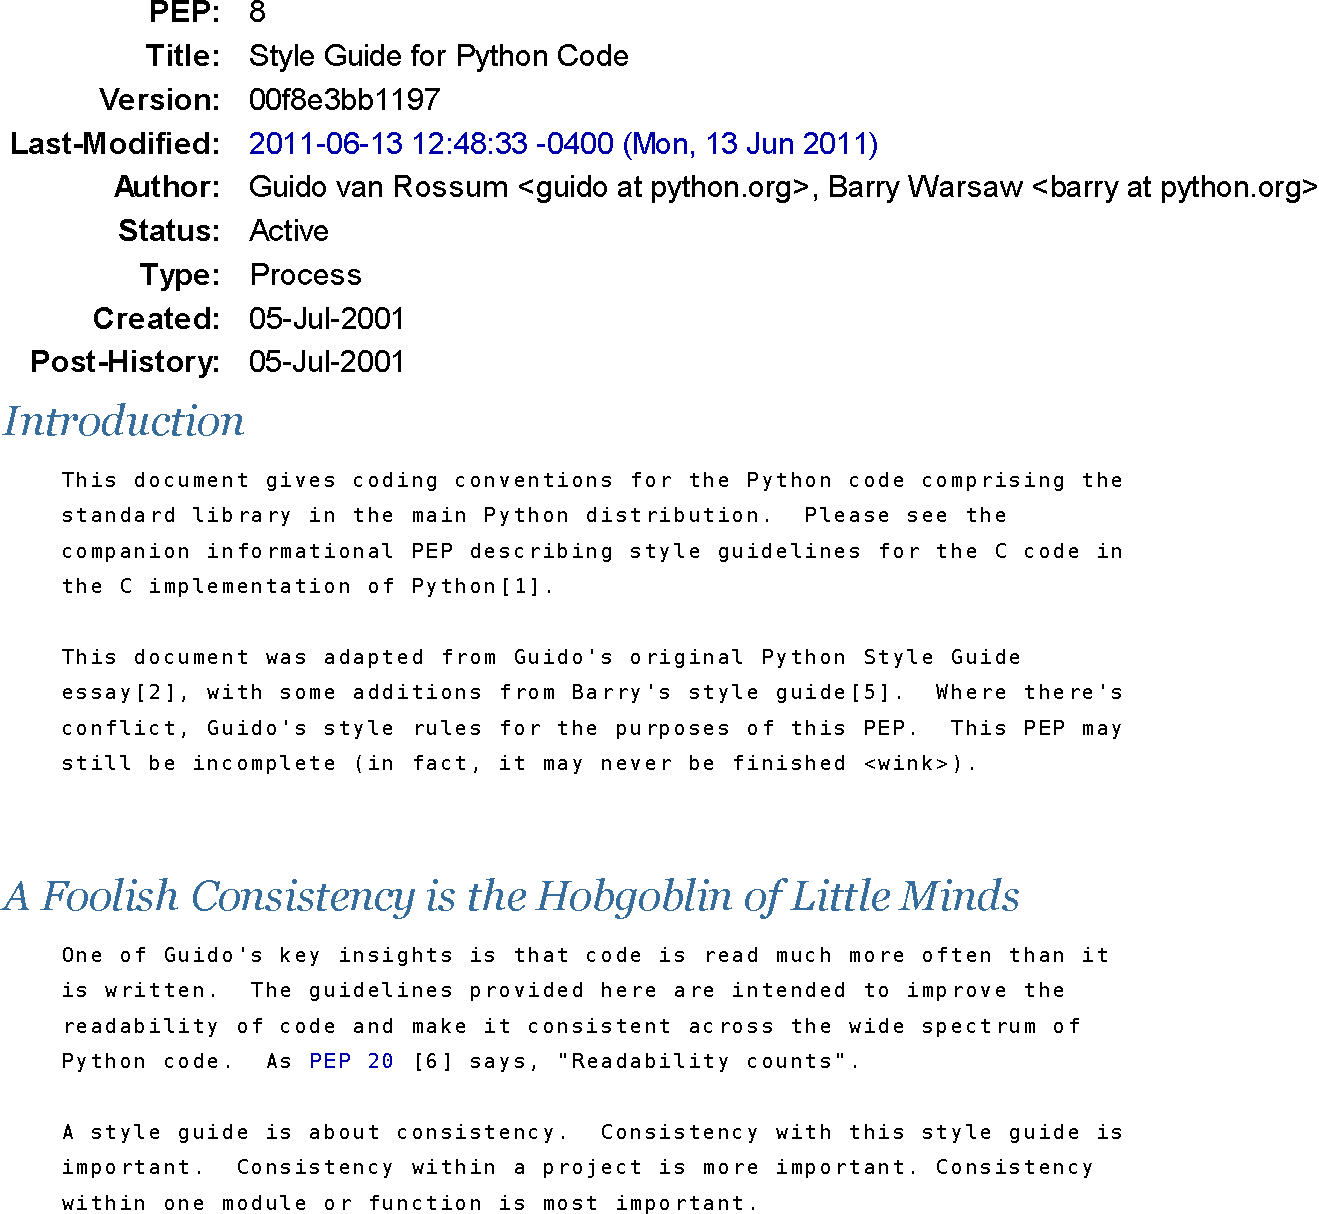
\includegraphics[width=\textwidth]{python/pep8}
  \caption{Excerpt from \ac{PEP} 8: Style Guide for Python Code}
\end{figure}

The Python project defines three types of \acp{PEP}.

\begin{description}

  \item[Standards Track PEP] The most common form of \acp{PEP} describes a
    feature proposal for the Python language. They always consist of a design
    document and a reference implementation.

  \item[Informational PEP] Unlike the Standards Track \ac{PEP}, this type for
    \ac{PEP} does not propose a new feature. It provides general guidelines or
    information about a certain issue of Python. However it does not
    necessarily reach consensus inside the Python community and so one is free
    to ignore Informational \acp{PEP}.

  \item[Process PEP] This kind of \ac{PEP} is quite like the Standards Track
    \ac{PEP}, except that it applies to other areas than the Python language
    and describes processes around Python. For example any guidelines, decision
    making processes, development workflow and so on are mostly a Process
    \ac{PEP}. Additionally any \acp{PEP} which describe other \ac{PEP}, for
    example how a \ac{PEP} should look like, will be seen as a Process \ac{PEP}
    too.

\end{description}

The \ac{PEP} process begins with a feature proposal for Python. While all
bigger proposals require a \ac{PEP}, the Python project suggests to submit
small change directly as a patch submission. A \ac{PEP} always has one or
several authors, who have the responsibility for it. They will begin by
submitting the \ac{PEP} to the Python project. More precisely it should be
presented to the python-ideas mailing list and subsequently sent to the
\ac{PEP} editors. The \ac{PEP} editors will assign a number and a category as
mentioned above. Additionally, new \acp{PEP} always start with the \emph{Draft}
status. From there, the \ac{PEP} workflow begins.

\begin{figure}[htbp]
  \centering
  \begin{tikzpicture}[auto]
   \node[rectangle, rounded corners, draw=black, text width=6.5em, minimum height=2em, text centered]
     (draft) {Draft};
   \node[below=0.5cm of draft, rectangle, rounded corners, text width=6.5em, minimum height=2em, text centered]
     (dummy) {};
   \node[below=0.5cm of dummy, rectangle, rounded corners, draw=black, text width=6.5em, minimum height=2em, text centered]
     (deferred) {Deferred};

   \node[right=1cm of draft, rectangle, rounded corners, draw=black, text width=6.5em, minimum height=2em, text centered]
     (accepted) {Accepted};
   \node[below=0.5cm of accepted, rectangle, rounded corners, draw=black, text width=6.5em, minimum height=2em, text centered]
     (rejected) {Rejected};
   \node[below=0.5cm of rejected, rectangle, rounded corners, draw=black, text width=6.5em, minimum height=2em, text centered]
     (withdrawn) {Withdrawn};

   \node[right=1cm of accepted, rectangle, rounded corners, draw=black, text width=6.5em, minimum height=2em, text centered]
     (final) {Final};
   \node[below=0.5cm of final, rectangle, rounded corners, draw=black, text width=6.5em, minimum height=2em, text centered]
     (replaced) {Replaced};
   \node[below=0.5cm of replaced, rectangle, rounded corners, draw=black, text width=6.5em, minimum height=2em, text centered]
     (active) {Active};

   \draw[draw, -latex] ($(draft.south) - (1cm,0)$) -- ($(deferred.north) - (1cm,0)$);
   \draw[draw, -latex] ($(deferred.north) - (0.5cm,0)$) -- ($(draft.south) - (0.5cm,0)$);
   \path[draw, -latex] ($(draft.south) + (0.5cm,0)$) |- (rejected);
   \path[draw, -latex] (draft) |- ($(withdrawn.west) + (-0.5cm,0.8cm)$) |- (withdrawn.west);

   \draw[draw, -latex] (draft.east) -- (accepted.west);
   \draw[draw, -latex, dashed] (accepted.south) -- (rejected.north);

   \draw[draw, -latex] (accepted.east) -- (final.west);
   \draw[draw, -latex, dashed] (final.south) -- (replaced.north);
  \end{tikzpicture}
  \caption{Possible paths of the status of \acp{PEP}}
\end{figure}

\begin{description}

  \item[Draft] This is the default state of any new \ac{PEP} on submission, as
    described above.

  \item[Deferred] A \ac{PEP} Editor can always, instead of assigning the Draft
    status, defer a \ac{PEP}. Reasons for a deferral could be duplication,
    being poorly written, lack of motivation by the author or not being in line
    with the Python philosophy.

  \item[Accepted] A \ac{PEP} will be able to get this status assigned, if all
    \ac{PEP} criteria are matched. This includes a precise formulation of the
    \ac{PEP}, not breaking backwards compatibility and finally be accepted by
    the \ac{BDFL}. However the criteria are not set in stone and basically a
    \ac{PEP} just have to be accepted by the \ac{BDFL} to get accepted.

  \item[Rejected] At this stage a \ac{PEP} can still be rejected. Mostly this
    status gets assigned, if it turns out that the original idea did not fit
    the Python project that well. But basically it is just a option to drop a
    \ac{PEP} even, after it was either accepted or not deferred.

  \item[Withdrawn] A \ac{PEP} can also always be withdrawn by the author of a
    \ac{PEP}. This could help if an author does not want to work on a \ac{PEP}
    anymore, for example because there is a better solution available.

  \item[Final] Once a \ac{PEP} has been accepted and has a reference implementation
    available, it can get the status Final by the \ac{BDFL}.

  \item[Replaced] Mostly for Informational \acp{PEP}, subsequent versions can
    replace a \ac{PEP}. In this case the original \ac{PEP} would be marked as
    Replaced and superseded by the new \ac{PEP}.

  \item[Active] Informational and Process \ac{PEP} can also be marked as Active, if
    they never will be completed. For example \ac{PEP} 1 \cite{Warsaw2000}, which
    describes the process of \acp{PEP} has it's status set to Active, as it is
    continually improved and adapted to new workflows.

\end{description}

\begin{figure}[htbp]
  \centering
  \includegraphics[width=0.8\textwidth]{python/authors_by_month}
  \caption{Amount of distinct authors of CPython over time}
\end{figure}

% }}}

% }}}


\cleardoublepage
\section{PHP Project Analysis} % {{{
\label{sec:PHP Project Analysis}

\marginpar{
\includegraphics[width=\marginparwidth]{php/logo}}

\subsection{Introduction} % {{{
\label{sub:Introduction}

PHP is a server side, interpreted programming language designed for web
applications and development \cite{PHPIntro}. As such, it requires a web server
with a connected PHP installation, though it can also be used with a command
line interface. It is widely available for all major platforms and is licenced
under the PHP Licence \cite{PHPManual}. It is worth noticing, that while it is
a Free Software licence, it is incompatible to the widely used \ac{GPL}. PHP
comes with an extensive standard library and supports many programming
paradigms, such as object oriented, imperative or procedural programming
styles. The abbreviation PHP originally stood for Personal Home Page
\cite{PHPHistory}. With PHP version 3, the project changed it's name to PHP
Hypertext Processor. PHP is a very popular programming language for web
development and featuring a large number of websites
\cite{PHPW3Techs,PHPStats}.

% }}}

\subsection{History} % {{{
\label{sub:History}

In 1994, Rasmus Lerdorf created the first version of PHP for his own website,
naming the program Personal Home Page Tools \cite{PHPHistory}. He published the
bundle one year later, after rewriting the original version. That also included
the first name change to FI (Forms Interpreter) and then to Personal Home Page
Construction Kit the same year. At that time, PHP could be considered as a
advanced programming interface.

However, it received another makeover in 1996, combining the two previous names
to PHP/FI. This time, PHP truly began to evolve to a full featured programming
language. It included several modules for database or browser interaction. This
version was also known as PHP/FI 2.0. Following a popularity boom in 1997 and
1998 it reached it's limitations due to the design of the project and by being
almost solely developed by Lerdorf.

In 1997 Andi Gutmans and Zeev Suraski rewrote the PHP interpreter and
approached Lerdorf discussing the problems PHP had at that time. Together, they
rewrote and redesigned the language and also changed the name to PHP Hypertext
Processor. Version 3.0 of PHP was then released in 1998 and replaced PHP/FI 2.0
completely. On of the most important features of the new approach was to
provide an interface for modules, which can be used directly from the
programming language.

The design of the language was improved further in 1998 improving performance
and the modularity of modules and code. The new engine was called Zend Engine
and provided the core of PHP 4.0, which was released in 2000.

Four years later, PHP 5 was released featuring the successor Zend Engine 2.0.
This release was incompatible to the previous 4.0 version and a large
initiative was planned to promote the transition from PHP 4 to PHP 5.

% }}}

\subsection{Community} % {{{
\label{sub:Community}

The PHP project consists of a large user and developer community
\cite{Magnusson2010}. Additionally to the PHP interpreter, there are many
people working on PHP extensions and components, which get distributed
alongside the standard interpreter.

The PHP community provides a large amount of conferences and workshops to meet
in person and work together on PHP. While the International PHP conference was
the first of it's kind in 2001 \cite{PHPConferences}, there are many
opportunities to meet other PHP contributors. A lot of local PHP User Groups
exist and provide weekly or monthly meetings and meet-ups such as workshops.

Most of the communication inside the PHP project is done through mailing lists
\cite{Magnusson2010}. It has mailing lists for most aspects of the project,
however the most important is the internals mailing list. Most of the
development process, future ideas and new contributions are handled over that
list. Of course, there are also several \ac{IRC} channels and blogs of PHP
developers available.

\begin{figure}[htbp]
  \centering
  \includegraphics[width=0.9\textwidth]{php/commits_by_author}
  \caption{Monthly activity of the most active PHP Developers}
\end{figure}

Officially, there is no categorizing of developers and everyone is treated
equally. However the project uses a concept named karma, which basically means
that one increases his karma by contributing to the project with code,
discussions and new ideas \cite{Magnusson2010}. Furthermore, several people are
responsible for different parts of the code or modules and can be classified
using those criteria \cite{PHPCredits}.

\begin{figure}[htbp]
  \centering
  \includegraphics[width=0.9\textwidth]{php/commits_by_year}
  \caption{Yearly overview of commits to PHP}
\end{figure}

\begin{description}

  \item[Developer] One is able to call himself a PHP Developer, once he gets a
    PHP Subversion account. According to the PHP community, an account needs to
    be earned, which basically means that one has to provide several patches
    and contributions to the PHP project first. Once one has shown enough
    commitment, he can apply for an account. The account however will be only
    granted if a reference person approves.

  \item[Module Author] Each developer has the possibility to become a module
    author. This role has the responsibility for a certain PHP module, which
    gets distributed with the PHP release. Examples for such modules are
    database or imaging modules. For each module, there can be more than one
    module authors, who share the responsibility.

  \item[PHP Author] This role defines a certain section of the PHP interpreter
    and it's responsibility for it. It is quite similar to the module author
    role, except that it covers only PHP itself.

  \item[Language Designer] Currently only Rasmus Lerdorf, Andi Gutmans and Zeev
    Suraski hold this role. They are the only who can actively change the
    programming language syntax and concepts.

\begin{figure}[hbtp]
  \centering
  \includegraphics[width=\textwidth]{php/punchcard}
  \caption{Time based view on commits of contributors}
\end{figure}

\end{description}

% }}}

\subsection{Release Process} % {{{
\label{sub:Release Process}

In 2010, the PHP project set up a new release plan with detailed information
about how the release process should work \cite{PHPRelease}. Before,
individuals decided when a release happened and which features it included. The
new release cycle features two Release Managers, who are voted by PHP
Developers and are managing the release process. The PHP project uses a scheme
with three numbers for releases: major, minor and micro. Major releases get
published quite seldom, can break backwards compatibility and are planned a
long time in advance. Minor releases can have new features and bug fixes,
however backwards compatibility must be kept. Micro release are bugfix only
releases where backwards and API compatibility must be kept. Each major release
is followed by a number of minor releases, which themselves are followed by a
number of micro releases.

\begin{figure}[htbp]
  \centering
  \includegraphics[width=\textwidth]{php/releases}
  \caption{Major Releases of PHP}
\end{figure}

Starting with PHP 5.4 a major or minor release will get published each year. Each
yearly release is then followed by a number of micro releases for 2 years,
which contains bug fixes only. After that period, only micro releases with
security relevant fixes will get published.

\begin{figure}[htbp]
  \centering
  \includegraphics[width=0.9\textwidth]{php/release_plan}
  \caption{Preliminary PHP release cycle}
\end{figure}

% }}}

\subsection{Development} % {{{
\label{sub:Development}

Most of the development process is handled over the PHP mailing lists
\cite{PHPRelease,Magnusson2010,PHPVoting}. Not every patch however needs to be
discussed and approved first, minor features or changes often get directly
committed to the repository. Though every change gets through a peer review
process, where other developers review the made changes. Every change gets
reviewed by other developers, who in case the need arises, discuss the change
on the developers mailing list. They then often result in a more comprehensive
change or in new features.

\begin{figure}[htbp]
  \centering
  \includegraphics[width=0.8\textwidth]{php/commits_by_month}
  \caption{Amount of commits per month of Core Contributors}
\end{figure}

To help the development and decision process, the PHP project keeps track of
new ideas, features and proposals through so called \ac{RFC} \cite{PHPRFC}.
Those are documents which describe the new feature and it's rationale. A
\ac{RFC} document is always owned by at least one person, who is responsible
for it. The \ac{RFC} process begins with the author's submission of the
\ac{RFC} to the PHP wiki and an announcement to the internals mailing list.
Depending on the importance and affected sections of the PHP project, the
following discussion period is set to a minimum of one to two weeks. It can be
longer however, but not shorter \cite{PHPVoting}.

After the discussion period has passed, the author can either call for a vote
or extend the discussion period as needed \cite{PHPVoting}. The vote is
announced on the mailing list and followed by a voting period which should be
at least one week, but can be extended if required.

Depending on the importance of a \ac{RFC}, it needs either 2/3 of all votes or
\unit[50]{\%} plus one to get accepted. The importance is defined by whether it
actually changes the syntax or behaviour of the PHP language and is therefore
irreversible or not. A failed proposal can be resurrected at least six months
after the last vote or if the author makes considerably large changes to the
\ac{RFC}. There is no definition by the PHP project, what considerably large
changes constitute, however the opinion is that it should be changed in a
matter, that it significantly can change a vote's outcome.

\begin{figure}[htbp]
  \centering
  \begin{tikzpicture}[auto]
   \node[rectangle, rounded corners, draw=black, text width=6.5em, minimum height=2em, text centered]
     (draft) {Draft};
   \node[below=0.5cm of draft, rectangle, rounded corners, text width=6.5em, minimum height=2em, text centered]
     (dummy) {};
   \node[below=0.5cm of dummy, rectangle, rounded corners, draw=black, text width=6.5em, minimum height=2em, text centered]
     (withdrawn) {Withdrawn};

   \node[right=1cm of draft, rectangle, rounded corners, draw=black, text width=6.5em, minimum height=2em, text centered]
     (discussion) {Discussion};
   \node[below=0.5cm of discussion, rectangle, rounded corners, draw=black, text width=6.5em, minimum height=2em, text centered]
     (accepted) {Accepted};
   \node[below=0.5cm of accepted, rectangle, rounded corners, draw=black, text width=6.5em, minimum height=2em, text centered]
     (implemented) {Implemented};

   \node[right=1cm of discussion, rectangle, rounded corners, draw=black, text width=6.5em, minimum height=2em, text centered]
     (voting) {Voting};
   \node[below=0.5cm of voting, rectangle, rounded corners, draw=black, text width=6.5em, minimum height=2em, text centered]
     (declined) {Declined};

   \path[draw, -latex] (draft) -- (discussion);
   \path[draw, -latex] (discussion) -- (voting);
   \path[draw, -latex] ($(discussion.south) - (0.5cm,0)$) |-+(0,-0.2cm)-| (withdrawn);
   \path[draw, -latex] ($(voting.south) - (0.5cm,0)$) |-+(0,-0.2cm)-| (accepted);
   \path[draw, -latex] ($(voting.south) + (0.5cm,0)$) -- ($(declined.north) + (0.5cm,0)$);
   \path[draw, -latex] (accepted) -- (implemented);
   \path[draw, -latex] (declined.south) -- ++(0,-0.4cm) -- 
   ([yshift=-0.4cm, xshift=0.4cm] declined.south east) --
   ([yshift=0.4cm, xshift=0.4cm] voting.north east) -| (draft.north);
  \end{tikzpicture}
  \caption{Possible paths of the status of \ac{RFC} documents}
\end{figure}

All PHP developers are allowed to vote and if needed, representatives from
the PHP community, such as participants of PHP related discussions or
developers of PHP appendant projects can participate in the
voting process. Those however have to be chosen by PHP developers
\cite{PHPWhoVote}.

During the whole development process, a \ac{RFC} has a status assigned, which can be
one of the following \cite{PHPRFC}.

\begin{description}

  \item[Draft] Once a \ac{RFC} gets submitted to the PHP wiki, it gets this
    status assigned. The Draft status means, that the \ac{RFC} is not ready yet
    for a discussion, however it can be improved by other people as well and a
    preliminary discussion can be started.

  \item[Discussion] Once the author of a \ac{RFC} announces it for discussion,
    it gets this status assigned. As previously described, the discussion phase
    starts with this status.

  \item[Voting] After the discussion phase the voting phase begins. While
    developers can vote for or against the \ac{RFC}, the Voting status gets
    assigned including a link to the voting site.

  \item[Accepted] Once a voting was successful, the \ac{RFC} is accepted and
    will be implemented or taken in action in near future.

  \item[Declined] If the majority voted against the \ac{RFC}, it gets declined.
    After six months and several changes to it, the author can resubmit it.

  \item[Implemented] If the voting was successful, the \ac{RFC} will get
    implemented or taken in action if it describes a community process.

  \item[Withdrawn] The author can withdraw the \ac{RFC} without calling for a
    vote if he thinks the \ac{RFC} is irrelevant or won't pass a vote.

\end{description}

\begin{figure}[htbp]
  \centering
  \includegraphics[width=0.8\textwidth]{php/authors_by_month}
  \caption{Amount of distinct authors of PHP over time}
\end{figure}

% }}}

% }}}


\cleardoublepage
\section{GNOME Project Analysis} % {{{
\label{sec:GNOME Project Analysis}

\marginpar{
\includegraphics[width=\marginparwidth]{gnome/logo}}

\subsection{Introduction} % {{{
\label{sub:Introduction}

GNOME is a desktop environment for UNIX based systems. It is composed by a
collection of tools and programs including a desktop shell in order to provide
all the essential utilities a user might need when working with a computer.
Officially, GNOME is part of the GNU project and licensed under the \ac{GPL}
and the \ac{LGPL}. The name GNOME was initially an acronym for \emph{GNU
Network Object Model Environment}, however that acronym was dropped. The GNOME
project targets for ease of use and user friendliness and therefore aims for
coherent and good user interfaces \cite{GNOMEHIG}, accessibility,
internationalization, regular releases and good support for users and
developers. GNOME is a modular project, meaning that it consists of several so
called modules, which can be either applications, libraries or utilities. Since
the release of GNOME 3, the modules were reorganized into a GNOME core suite
and a GNOME apps suite. GNOME core provides everything to run a basic desktop
system and will therefore be analyzed in this context.

\begin{figure}[htbp]
  \centering
  \includegraphics[width=0.9\textwidth]{gnome/commits_by_author}
  \caption{Monthly activity of the most active GNOME core developers}
\end{figure}

% }}}

\subsection{History} % {{{
\label{sub:History}

GNOME was first announced and started in 1997 by Miguel de Icaza and Federico
Mena Quintero as a counterpart to KDE
\cite{German2003,GNOMEAbout,GNOMEAnnouncement}. Both were attending university
at that time when they set their aim to produce a desktop environment using
only free software technologies. KDE relied on the Qt widget toolkit, which at
that time was licensed under a proprietary software license. Instead of using
Qt, the GTK+ toolkit originally developed for the GIMP graphics editor was
used. The GNOME project quickly grew into a large project which nowadays is the
most popular desktop environment for UNIX type operating systems. The desktop
as well as the developer technologies can be found on workstations and large
enterprises but also on mobile devices. With the recent GNOME 3 release the
project did a major overhaul with a significant redesign of the desktop
environment and an entirely new user interface \cite{GNOMEPress}.

% }}}

\subsection{Community} % {{{
\label{sub:Community}

The GNOME project consists of a large user and developer community. While there
were about 3500 people contributing to GNOME and it's applications, there is
also a big community around the project, which for example uses GNOME
technologies such as GStreamer or GTK+ \cite{GNOMEAbout,GNOMETeams}.

Most of the communication inside the project is handled over mailing lists and
\ac{IRC} channels. Quite every GNOME module has a dedicated mailing list or
\ac{IRC} channel. Global decisions are mostly handled over the desktop-devel
mailing list. Additionally blogs are widely spread in the GNOME community and
contributors often write blog posts about achieved things, wishes and starting
discussions.

Next to several hackfests each year, the community holds a yearly conference
under the name GUADEC. It stands for GNOME User and Developer European
Conference, and while the conference only took place in Europe so far it is
nevertheless considered an international conference \cite{GNOMEGUADEC}.

\begin{table}
  \centering
  \begin{tabularx}{\textwidth}{lXl}
    \toprule
    \tableheadline{Event}                   & \tableheadline{Venue}       & \tableheadline{Date} \\
    \midrule
    GUADEC \MakeUppercase{\romannumeral 1}  & Paris, France               & 2000 \\
    GUADEC \MakeUppercase{\romannumeral 2}  & Copenhagen, Denmark         & 2001 \\
    GUADEC \MakeUppercase{\romannumeral 3}  & Seville, Spain              & 2002 \\
    GUADEC \MakeUppercase{\romannumeral 4}  & Dublin, Ireland             & 2003 \\
    GUADEC \MakeUppercase{\romannumeral 5}  & Kristiansand, Norway        & 2004 \\
    GUADEC \MakeUppercase{\romannumeral 6}  & Stuttgart, Germany          & 2005 \\
    GUADEC \MakeUppercase{\romannumeral 7}  & Vilanova i la Geltrú, Spain & 2006 \\
    GUADEC \MakeUppercase{\romannumeral 8}  & Birmingham, England         & 2007 \\
    GUADEC \MakeUppercase{\romannumeral 9}  & Istanbul, Turkey            & 2008 \\
    Desktop Summit                          & Gran Canaria, Spain         & 2009 \\
    GUADEC \MakeUppercase{\romannumeral 10} & The Hague, Netherlands      & 2010 \\
    Desktop Summit                          & Berlin, Germany             & 2011 \\
    GUADEC \MakeUppercase{\romannumeral 11} & La Coruña, Spain            & 2012 \\
    \bottomrule
  \end{tabularx}
  \caption{Previous and planned GNOME conferences}
\end{table}

Due to the large and modular composition of the GNOME project, there are
similar roles for each module. Only very few teams and roles stand above all
modules. In this respect the developer community can be very much be seen as a
flat structure \cite{GNOMETeams,German2003,GNOMEDesignTeam,GNOMEReleaseTeam}.

\begin{description}

  \item[Committer] Any person who contributed a reasonable amount of
    improvements to the GNOME project or to a single module can become a
    committer. A committer has full read and write access to all GNOME
    repositories. Though each commit will be reviewed and approved by the
    maintainer of the module. To get such an account, one has to make a formal
    request to the Accounts Team along with one or several vouchers who can
    confirm your contributions to the GNOME project. Every module maintainer or
    translation team leader can act as a voucher. Furthermore will the voucher
    be responsible for the actions of the requesting person on the
    repositories.

  \item[Maintainer] Every module has one or more maintainers who will be
    responsible for releases, reviewing patches and the direction of a module.
    They are the main contact for the community and therefore act as the leader
    of a certain module. A single module can be maintained by multiple
    maintainers and one maintainer can maintain several modules. To become a
    maintainer one has either to create a new module which gets incorporated
    into the GNOME project or be asked by another maintainer.

  \item[Release Team] This team is responsible for a wide range of tasks
    concerning the development process of the GNOME project. Their tasks
    include for example creating a development schedule, making and publishing
    releases, approving or rejecting freeze break requests and defining the
    module list for GNOME releases. The team size is not fixed and can vary
    over time. Membership is only done through an invitation and often only
    when one person leaves the team. The leaving person may recommend a new
    team member on which the team will decide.

  \item[Design Team] Since GNOME 3 the Design Team holds a much more important
    role in the GNOME project as they primarily define the design of the GNOME
    user experience. This is done by designing the user interface and workflow
    of GNOME modules. Additionally they play an important part in the feature
    based development process.

  \item[GNOME Founders] Miguel de Icaza and Federico Mena Quintero, the
    original GNOME founders, played an important role in the first years of the
    GNOME project. Nowadays however they are more active in projects around
    GNOME technologies and often act as visionaries.

\end{description}

\begin{figure}[htbp]
  \centering
  \includegraphics[width=0.9\textwidth]{gnome/commits_by_year}
  \caption{Yearly overview of commits to GNOME core}
\end{figure}

% }}}

\subsection{Release Process} % {{{
\label{sub:Release Process}

The GNOME project uses a version naming scheme with three numbers however
distinguishes only between major and minor releases
\cite{GNOMEDevelopmentSchedule,GNOMESchedule}. The numbers are however
nevertheless called major, minor and macro numbers. An incrementation of the
first number only happens when the project does a ground-breaking change, such
as using GTK+2 for GNOME 2.x or the new user experience with the GNOME shell
and GTK+3 for GNOME 3.x. For the minor version number the GNOME project uses
odd numbers indicating an unstable series and even numbers for stable releases.
For example the unstable 3.1.x series will become into the stable 3.2.x release
series.

\begin{figure}[htbp]
  \centering
  \includegraphics[width=\textwidth]{gnome/releases}
  \caption{Major Releases of GNOME}
\end{figure}

\begin{figure}[htbp]
  \centering
  \includegraphics[width=\textwidth]{gnome/punchcard}
  \caption{Time based view on commits of Core contributors}
\end{figure}

The release schedule is fixed and every six months a new major release will
appear. To achieve this, a release schedule is published by the release team
every six months \cite{GNOMEDevelopmentSchedule}. Over the years it stayed
mostly the same, while a few minor changes might occur to comprise conferences
or holidays. The release schedule includes future stable minor releases, the
two schedules overlap.

Each stable release series consists of at least three releases which will be
named with x.y.0 to x.y.2. Of course, a module maintainer can decide to provide
more stable releases \cite{GNOMEReleaseTeam}. The unstable series consists of
eight releases which are distributed over six months. The schedule furthermore
includes proposal and freeze periods which will be described in the following
\cite{GNOMEDevelopmentSchedule,GNOMESchedule}.

\begin{figure}[htbp]
  \centering
  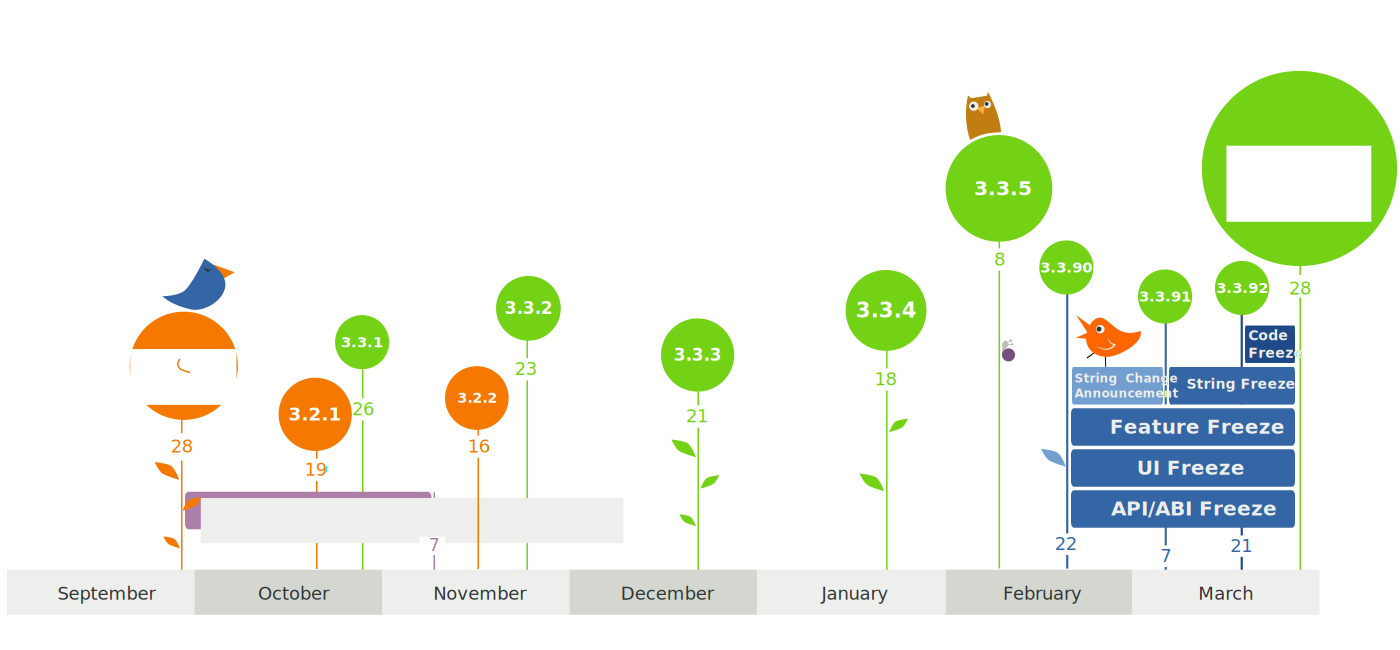
\includegraphics[width=\textwidth]{gnome/gnome-timeline}
  \caption{Release Schedule which will lead to GNOME 3.4}
\end{figure}

\begin{description}

  \item[Feature proposal period] After a major release gets published the
    feature proposal period starts. GNOME developers can propose features for
    the next major release and discuss them with the community. Approximately a
    month later, when the first unstable release gets published, the proposal
    period ends. Around two weeks later the release team meets and decides
    about proposed features with the community input up to this point.

  \item[The Freeze] With the release of the first beta release the first freeze
    is in action. No user interface changes, new features, developer API
    changes are allowed without approval from the release team. This excludes
    of course bug fixes. Additionally new translatable strings must be
    announced to the translation and documentation team.

  \item[String Freeze] With the second beta release no string changes are
    allowed anymore without confirmation of both the release and translation
    team.

  \item[Hard Code Freeze] With the release of the release candidate no source
    code changes are allowed without approval of the release team.
    Documentation and translation however can continue. After publishing the
    next major GNOME release the Hard Code Freeze ends but all other freezes
    remain in action for the stable series.

\end{description}

\begin{figure}[htbp]
  \centering
  \includegraphics[width=0.8\textwidth]{gnome/commits_by_month}
  \caption{Amount of commits per month of Core contributors}
\end{figure}

% }}}

\subsection{Development} % {{{
\label{sub:Development}

Before the release of GNOME 3, the release team would decide together with the
community about the inclusion of new modules. The development of each module
was planned an executed by the maintainers. Since GNOME 3, the development
workflow changed into a more design driven development approach. This means
that all new features concerning user interface or applications have to go
through the design team \cite{GNOMEDesignTeam}. This leads to a consistent
process which delivers a uniform user interface. However the design team has no
sort of decision making authority and a maintainer can ignore the design
proposal by the design team.

Next to the design driven approach the module inclusion changed to a feature
inclusion approach \cite{GNOMEFeatures3.4,GNOMERoadMap}. Every GNOME
contributor can create a feature proposal in which he describes a feature he
would like to see in the next stable GNOME release. A feature proposal is
composed by a description of the problem which will be solved, one or more
authors, a list of involved parties and the current status of the proposal. All
of these fields are required and a feature will not be accepted until all are
filled out. After each major release and until about a month later, one can
propose a feature for inclusion. The community has time to discuss the features
and improve them for roughly one and a half months. After that time the release
team will meet and depending on the feedback of the community decide about the
inclusion of each feature. If a feature gets accepted the author of the feature
will be the leader of it and responsible for the completion. With the release
of the first beta release and the establishment of the Feature, UI and
\ac{API}/\ac{ABI} Freeze the feature has to be finished and working. If not, it
may be postponed to the next major release.

\begin{figure}[htbp]
  \centering
  \includegraphics[width=0.8\textwidth]{gnome/authors_by_month}
  \caption{Amount of distinct authors of GNOME core over time}
\end{figure}

% }}}

% }}}


\cleardoublepage
\section{KDE Project Analysis} % {{{
\label{sec:KDE Project Analysis}

\marginpar{
\includegraphics[width=\marginparwidth]{kde/logo}}

\subsection{Introduction} % {{{
\label{sub:Introduction}

KDE is a desktop environment designed to run on UNIX based systems as well as
Microsoft Windows and Mac OS X systems \cite{KDEPress,KDEAbout}. Since 2010 and
the release of KDE 4.4 the project is known as \ac{KDE SC}. It is composed by
the desktop environment named Plasma Desktop and several core application for
the daily needs. \ac{KDE SC} is licensed under the \ac{GPL} and \ac{LGPL}. The
name was originally an acronym for Kool Desktop Environment and later for K
Desktop Environment, however it is no longer in use. KDE is a modular project
consisting of several libraries which allow developer to build their programs
around the platform. As the KDE project and the \ac{KDE SC} stand for a wide
range of technologies and applications, this analysis will be limited to the
core of the \ac{KDE SC}, also known as KDE Base.

% }}}

\subsection{History} % {{{
\label{sub:History}

KDE was first announced started by Matthias Ettrich in 1996 as a desktop
environment for end users with the same feel and look for all applications
\cite{KDEAnnouncement}. The name KDE was more a word play with the existing
Common Desktop Environment (CDE), which was highly popular at that time. As the
graphical library, Matthias Ettrich chose the Qt framework which was and is
developed by the company Trolltech. KDE 1.0 was then released in 1998
\cite{KDEHistory}. At the same time, Trolltech dual licensed the framework
under the Q Public License (QPL) and a proprietary software licence. However,
it was debated if that license was compatible with the \ac{GPL} and in 2000 the
framework was licenced under the \ac{GPL} which ceased the criticism.

In 2009 the KDE project renamed the project to \ac{KDE SC} and redefined the
project as a community which delivers free software for user interfaces by
emphasizing the KDE technologies \cite{KDESC}. All software created with KDE
technologies will be a KDE project. However \ac{KDE SC} only contains projects
which come out from the project itself and share a common release cycle.

\ac{KDE SC} 4 was a new approach to the desktop metaphor and created a new user
experience for users. The centerpiece is the Plasma Workspace which exists for
several devices, such as for desktop computers, netbook, tablets and
smartphones.

% }}}

\subsection{Community} % {{{
\label{sub:Community}

The KDE project is one of the largest FOSS projects and according to the
project the second largest after the Linux Kernel \cite{KDEPress}. There are
about 1800 active contributors to the project and it's surroundings and is used
by over a million people. Also, the community spans around projects basing on
KDE technologies.

Most of the communication in the KDE project is done via mailing lists, most
importantly kde-devel and kde-core-devel
\cite{KDEProjectManagement,KDEContribute}. While the first one is mostly used
for communication by application developers, the latter one is for
communication of the KDE core project. Furthermore communication can happen
over \ac{IRC} channels, blogs or forums.

The most important KDE conference is the annual Akademy which is hold at
different locations in Europe \cite{KDEHistory}. The first KDE conferences were
however named after the current release which started with KDE One in 1997.
That is also the reason, why the conferences did not happen annually at that
time. Not until 2004 it changed the name to Akademy. Beginning with 2009 the
project incorporates the conference into the Desktop Summit which is a
collaboration with the GNOME project.

\begin{table}
  \centering
  \begin{tabularx}{\textwidth}{lXl}
    \toprule
    \tableheadline{Event}   & \tableheadline{Venue}           & \tableheadline{Date} \\
    \midrule
    KDE One                 & Arnsberg, Germany               & 1997 \\
    KDE Two                 & Erlangen, Germany               & 1999 \\
    KDE Three Beta          & Trysil, Norway                  & 2000 \\
    KDE Three               & Nürnberg, Germany               & 2002 \\
    Kastle                  & Nové Hrady, Czech Republic      & 2003 \\
    aKademy                 & Ludwigsburg, Germany            & 2004 \\
    aKademy                 & Málaga, Spain                   & 2005 \\
    aKademy                 & Dublin, Ireland                 & 2006 \\
    aKademy                 & Glasgow, Scotland               & 2007 \\
    Akademy                 & Sint-Katelijne-Waver, Belgium   & 2008 \\
    Desktop Summit          & Gran Canaria, Spain             & 2009 \\
    Akademy                 & Tampere, Finland                & 2010 \\
    Desktop Summit          & Berlin, Germany                 & 2011 \\
    Akademy                 & Tallinn, Estonia                & 2012 \\
    \bottomrule
  \end{tabularx}
  \caption{Previous and planned KDE conferences}
\end{table}

Owing to the size of the KDE project it is organized around many independent
teams with a communication structure between them. There are few groups who
stand above those teams and only take care about coordinating the project
\cite{KDEDevelopmentModel,KDEProjectManagement}.

\begin{description}

  \item[Contributor] After having contributed to any KDE project for some time
    and planning to contribute in the future, a KDE Contributor account can be
    requested \cite{KDEContribute,KDEContributor}. In the request one must
    state why they are interested in having an account. The KDE sysadmin team
    will then check the application and grant an account or not.

  \item[Module Coordinator] As the KDE project is highly modular, quite each
    application or library has an independent team with it's own structure. A
    module coordinator plans and executes releases and the direction of a
    single module. As the teams are so diverse, there are many ways to become a
    module coordinator. The most obvious is of course by unweary contributions
    to a project.

\begin{figure}[htbp]
  \centering
  \includegraphics[width=0.9\textwidth]{kde/commits_by_author}
  \caption{Monthly activity of the most active KDE core developers}
\end{figure}

  \item[Core Team] One of the most important teams is the Core Team as it
    defines the overall direction the project is heading
    \cite{KDEProjectManagement}. There is no single person inside the team
    which takes the decision, instead the team takes a decision by discussing
    the issue and coming up with a solution. The primary communication method
    is the kde-core-devel mailing list which is publicly readable, however an
    approval is required to join it. The KDE project does not define clear
    restrictions to membership and so a membership is by invite only after
    distinguishing or outstanding work for the KDE project.

  \item[Release Team] The actual release and the release schedules are provided
    and enforced by the Release Team \cite{KDEReleaseTeam}. It is composed by
    module coordinators and other release team members who actually do the
    releases. The Release Team makes sure that all modules are following the
    release schedule and are in a good shape. Also they decide on code freeze
    breaks and take decision about future features of a release.

  \item[KDE Founder] Matthias Ettrich, the founder of the KDE project is no
    longer actively involved in the project as he works full time on the
    underlying Qt framework. However he has still an important voice in the
    community and contributes indirectly to KDE by his role in the Qt project.

\end{description}

\begin{figure}[htbp]
  \centering
  \includegraphics[width=0.9\textwidth]{kde/commits_by_year}
  \caption{Yearly overview of commits to KDE base}
\end{figure}

% }}}

\subsection{Release Process} % {{{
\label{sub:Release Process}

The KDE project uses a version naming scheme with three numbers and
distinguishes between major and minor releases
\cite{KDEReleaseTeam,KDEReleaseSchedule,KDESchedule}. The numbers are called
major, minor and macro numbers. The major and minor number define major
releases while the macro number defines a maintenance release. Depending on
whether the major or minor number changes the release is a platform or standard
release. A platform release defines a new series of releases which can break
backwards compatibility to the previous platform release. They are often
planned a long time beforehand with usually also changing the used libraries or
switching their used versions. A standard release however has to maintain
backwards compatibility with it's series. They can have new features and user
interface changes, however a KDE application has to work on all releases of the
same platform. Maintenance releases are not allowed to have new features,
however bug fixes and small enhancements are allowed. Beginning with \ac{KDE
SC} 4 the cycle changed to a major release every six months and a maintenance
release roughly every month except when a major release comes out.

\begin{figure}[htbp]
  \centering
  \includegraphics[width=\textwidth]{kde/releases}
  \caption{Platform and Standard Releases of KDE}
\end{figure}

\begin{figure}[htbp]
  \centering
  \includegraphics[width=\textwidth]{kde/punchcard}
  \caption{Time based view on commits of Core contributors}
\end{figure}

To ensure the release schedule, the release team publishes a new release
schedule after each major release. The schedule includes all deadlines and
freezes which will lead to the next major release and includes future
maintenance releases. This means of course that two release schedules will
overlap until the month before the new major release. The following freezes and
releases are provided and enforced by the release team
\cite{KDEReleaseSchedule}.

\begin{description}

  \item[Soft Feature Freeze] Approximately three weeks before the first beta
    release no new features are allowed if they are not already approved as
    planned features. Not ready features have to be postponed to the next major
    release.

  \item[Dependency Freeze] Approximately two weeks before the first beta
    release no new or new dependency versions are allowed anymore. However it
    is possible to request an exception by the release team.

  \item[Soft Message, Soft API and Hard Feature Freeze] One week before
    the first beta release no new strings and changes to the existing messages
    can be made except corrections. Additionally the existing API should be
    almost finished and if changes are made they should be reported to the
    relevant teams. Lastly no new features can be added to the projects, even
    if they were planned for this release cycle.

  \item[Beta Release] Approximately two months before the major release the
    first beta release gets published. This is usually followed by a second
    beta release two weeks later.

  \item[Hard API, Message and Documentation Freeze] Five weeks before the
    major release the \ac{API}, translatable messages and the documentation
    must be finished and can't be changed anymore.

  \item[Release Candidate] Approximately a month before the final release the
    first release candidate will be published. Two weeks later the second
    release candidate follows.

  \item[Final Release] The final release will then be published three weeks after
    the last release candidate.

  \item[Minor Releases] A new minor release will be published each following
    month until the next major release gets published. This normally leads to
    four minor releases.

\end{description}

\begin{figure}[htbp]
  \centering
  \includegraphics[width=0.8\textwidth]{kde/commits_by_month}
  \caption{Amount of commits per month of Core contributors}
\end{figure}

% }}}

\subsection{Development} % {{{
\label{sub:Development}

During the development of a new major release, new project goals are set using
feature proposals \cite{KDEDevelopmentModel,KDEFAQ}. This normally happens
after each major release when KDE developers have the time to propose new
features for the next major release. Each feature must have an author who is
willing to do the implementation of that feature. This often limits the
features to projects of already contributing KDE developers. A KDE developer is
free to implement the feature by himself, however it often is accompanied by a
discussion with the specific team and several adjustments to the
implementation.

At the time of the soft feature freeze it is decided whether the feature will
be available for the upcoming major release or if it will be postponed to the
next major release. If the implementation already started and it is almost
finished, it can continue. Otherways it will be postponed. This development
process is a quite deliberate approach where people are free to implement what
they see missing in the project.

\begin{figure}[htbp]
  \centering
  \includegraphics[width=0.8\textwidth]{kde/authors_by_month}
  \caption{Amount of distinct authors of KDE base over time}
\end{figure}

% }}}

% }}}


\cleardoublepage
\section{Definition and Origin of the Catalogue} % {{{
\label{sec:Definition and Origin of the Catalogue}

To characterize the development process of FOSS project, the following
catalogue was established. By covering all listed points one a project should
have been analysed thoroughly and lead to a reasonable breakdown of all
projects.

\begin{description}

  \item[Description of the Project] A general description about the project
    should be provided to inform the reader about the goals and current state
    of a project.

  \item[Project Category] In order to provide methods to compare projects, the
    project category can help to contrast projects of the same and other
    categories. Examples are programming languages or content management
    systems.

  \item[Scope of Analysis] As FOSS projects often are hard to analyze due to
    their size and unclear definition of modules, the scope will be limited to
    a well known subset of the whole project.

  \item[License] Some projects use their own license and some use the well
    known General Public License. It is interesting to find out whether this
    makes any difference in the development process of a module.

  \item[History] As only projects with a quite long history are analyzed it
    makes sense to glance at the project's history.

  \begin{description}

    \item[Founders] In some projects, the original founders are still present
      and have a influential voice, in others the original authors are no
      longer involved. To analyzed this further, the authors have to be
      introduced and their role will be analyzed in the community part.

    \item[Project Age] Projects always need time to evolve and to find their
      best development process. As this needs time, the project age can give
      some information in what development process state this project is and
      how it will evolve in the future.

  \end{description}

  \item[Community] The people behind the project are the driving force. Without
    them, a project would not exist. Therefore it is important to analyze the
    diverse community of a project.

  \begin{description}

    \item[Size of the Community] An important measure is the approximate size
      of a community. Several structural changes inside the project can depend
      on this size.

    \item[Communication inside the Project] The communication is a vital thing
      in an open project. It is interesting to compare the different methods of
      communication in several projects depending on their development
      structure and size.

    \item[Conferences and Meet-ups] Meetings of developers are an important
      element of the development process in FOSS projects. Also it shows, that
      there is enough interest available to provide the money needed for
      preparing such events.

    \item[Roles] The development process is often defined and lead by important
      roles in the project. Also, depending on what role a person has in the
      project, his influence varies. 

    \item[Role of the Founders] In some projects the founders are still
      actively involved and in some not. Depending on that, the founders often
      have a very important role in the project development process.

  \end{description}

  \item[Release Process] In the FOSS world an often heard statement is that a
    new version will be released when it is ready. In fact however quite all
    projects have a certain release schedule or process they follow.

  \begin{description}

    \item[Version Naming] Each project provides a specific version naming
      scheme to which they adopt and which characterizes major, minor or bug
      fixing releases. This information is vital to understand the project's
      release schedule.

    \item[Characterization of Major and Minor Releases] Most projects provide
      some kind of major releases with new features which is often incompatible
      with previous releases, minor releases which mostly are backwards
      compatible and provide new features and finally bug fixing only releases.
      This however differs from project to project.

    \item[Release Schedule] Even if there are no fixed release cycles, most
      projects have nevertheless a release schedule in action. The release
      schedule defines deadlines and important steps in the process of creating
      a new release.

    \item[Important Steps in the Schedule] These often define freezes or
      specific points in time when all members of the project are restricted to
      for example not provide new code in order to increase the stability of
      the new release.

  \end{description}

  \item[Development] The actual development is closely interweaved with the
    release process and defines how and when the development of a project takes
    place.

  \begin{description}

    \item[Development Lead] In fact, most FOSS projects are lead by groups of
      people who define new features and lead the development process.
      Additionally there are hardly any projects which have a completely
      unstructured development process and have no development leaders in
      place.

    \item[Development Workflow] The actual development process as often defined
      by the project leaders provides ways and methods to propose and develop
      new features for the upcoming release.

    \item[Feature Inclusion Process] This inclusion process is used by some
      projects which defines process how and when new features and come into
      the project.

  \end{description}

\end{description}

% }}}

\section{PostgreSQL Project Analysis} % {{{

\marginpar{
\includegraphics[width=\marginparwidth]{postgresql/logo}}

The PostgreSQL project provides an \ac{ORDBMS} which runs on all major systems
such as Linux, UNIX, Microsoft Windows or Mac OS X
\cite{PostgreSQLAbout,PostgreSQLFAQ}. The group behind the project is known as
PostgreSQL Global Development Group which consists of several volunteers and
employed developers. PostgreSQL is quite popular amongst it's users and has won
several prizes for the best database management system \cite{PostgreSQLAwards}.
According to the project it is the leading \ac{FOSS} database system with
thousands of users and contributors \cite{PostgreSQLPressKit}.

\begin{description}

  \item[Project Category] PostgreSQL is a database management system, more
    specifically a \ac{ORDBMS} \cite{PostgreSQLAbout}.

  \item[Scope of Analysis] The PostgreSQL Core Distribution will be analyzed,
    which consists of the PostgreSQL database server, several tools and
    bindings around it \cite{PostgreSQLDownload}.

  \item[License] The PostgreSQL project makes use of the PostgreSQL license,
    which is a \ac{FOSS} license \cite{PostgreSQLFAQ,PostgreSQLLicense}. It
    only requires to maintain the copyright and licensing information in the
    licensed source code and therefore it is quite similar to a BSD license.

  \item[History] The project was started in 1986 by Lawrence A. Rowe and
    Michael R. Stonebraker at the University of California in Berkeley under
    the name POSTGRES \cite{PostgreSQLHistory}. Not until 1996 it was developed
    in a university style fashion trying to explore new areas in database
    management systems. It was then released as \ac{FOSS} by two students of
    Stonebraker with the new name PostgreSQL the adopted \ac{SQL}. It then
    received a big development boost and emerged to one of the leading
    \acp{ORDBMS}.

  \item[Community] The PostgreSQL project has a quite large community available
    which will be described in the following.

  \begin{description}

    \item[Size of the Community] According to the project there are 6 core team
      members, 38 major contributors and 42 contributors
      \cite{PostgreSQLContributors}. Adding no longer active persons the number
      sums up to around 140. The number of total contributors might however be
      higher, as the project only includes people who have made contributions
      over a long time.

    \item[Communication inside the Project] The communication mostly happens
      over mailing lists, although also \ac{IRC} channels exist. The most
      important mailing list for development is the pgsql-hackers mailing list
      \cite{PostgreSQLDevFAQ}.

    \item[Conferences and Meet-ups] The most important international conference
      is the annual PgCon which first happened in 2007 \cite{PostgreSQLEvents}.
      However there are a lot of local conferences and workshops available.

    \item[Roles] The developers are split into three groups
      \cite{PostgreSQLContributors}. The core team decides on the general
      direction of the PostgreSQL project as well as the release cycle and the
      releases. Major contributors are people who introduced or maintain big
      features to the project. The contributors are all other who provide
      patches to the project.

    \item[Role of the Founders] Michael R. Stonebraker and Lawrence A. Rowe did
      not follow the project when it was published as \ac{FOSS} in 1996
      \cite{PostgreSQLHistory}. They are therefore no longer actively involved
      in the project.

  \end{description}

  \item[Release Process] The used release process is highly structured and will
    be described in the following.

  \begin{description}

    \item[Version Naming] The PostgreSQL project uses a three digit number
      scheme which consists of a major, minor and micro number
      \cite{PostgreSQLVersioning}.

    \item[Characterization of Major and Minor Releases] The incrementation of a
      major or minor number defines a major release including new features and
      often backwards incompatible changes \cite{PostgreSQLVersioning}. Such a
      release occurs roughly once a year
      \cite{PostgreSQLDevelopment,PostgreSQLFAQ}. For each major release there
      exist a number of minor releases which are defined by incrementing the
      micro version number. Only bug and security fixes are allowed for those
      releases. Each major release is supported for five years by the
      PostgreSQL project. However in some cases the project can decide to drop
      support for a specific release if bugs cannot be resolved without risking
      the stability.

    \item[Release Schedule] As major releases occur every year, the project
      uses the same release schedule every year along with some minor
      improvements from the last years \cite{PostgreSQLDevelopment}. The
      release schedule gets planned and decided during the PgCon conference. It
      basically starts each June with a commit review in which possible patches
      might be included in the next major release. Such reviews, also known as
      Commit Fest happen four times each two months apart. In the month between
      an alpha release is published. After the last Commit Fest, more alpha
      releases can follow, if not beta releases are published. If no more
      critical errors are found several release candidates will be published
      which will lead to the next major release.

    \item[Important Steps in the Schedule] The Commit Fest are the only
      possibility to add new features to the project and are therefore a vital
      part of the development process
      \cite{PostgreSQLDevelopment,PostgreSQLCommitFest}. 

  \end{description}

  \item[Development] The development of the PostgreSQL project is closely
    entangled with the release process and will be described in the following.

  \begin{description}

    \item[Development Lead] The PostgreSQL project is mostly driven by the core
      team \cite{PostgreSQLDevFAQ,PostgreSQLFAQ,PostgreSQLContributors}. Quite
      all decisions are made by them as well as most new features and code
      contributions.

    \item[Development Workflow] Small patches are often submitted directly to
      the repository if they are done by a major contributor or a core team
      member \cite{PostgreSQLDevFAQ}. All other patches however have to be
      reviewed and therefore be sent to the pgsql-hackers mailing list. New
      features are proposed in the Commit Fests.

    \item[Feature Inclusion Process] The already mentioned Commit Fest is a
      periodic break in which no new development is done, however already
      existing patches are reviewed and get feedback
      \cite{PostgreSQLCommitFest}. Not only the core team does those reviews
      but also other developers. A single Commit Fest usually runs for about
      one month explaining the gap of one month between each Commit Fest. One
      such event is lead by a Commit Fest Manager who is responsible that all
      submitted patches will be reviewed. Often, a review results in a
      discussion on the mailing list and follows an acceptance, a return with
      feedback or a rejection. A patch can have several states, depending on
      whether it is in progress or if it is finished
      \cite{PostgreSQLCommitFestRunning}. If a patch is in progress, the
      following states might apply.

      \begin{description}

        \item[Needs Review] A patch is not reviewed and waiting for a review.

        \item[Waiting on Author] A new version of the patch is expected by the
          author.

        \item[Discussing Review Results] The review was done, however it is
          discussed on the mailing list.

        \item[Ready for Committer] The review was done and no issues were
          found. It is now waiting for a final review.

      \end{description}

      The in progress states of a patch are the following.

      \begin{description}

        \item[Returned With Feedback] The patch was reviewed and feedback was
          given. A new version of the patch is expected for the next Commit Fest.

        \item[Rejected] The patch was rejected and won't make it into the next
          major release.

        \item[Committed] The patch was applied and no remaining issues are
          assured.

      \end{description}

  \end{description}

\end{description}

% }}}

\section{MySQL/MariaDB Project Analysis} % {{{

\marginpar{
\includegraphics[width=\marginparwidth]{mariadb/logo}}

MySQL is according to the project the world's most used \ac{ORDBMS}
\cite{MySQLSun}. It runs on all major platforms and is widely used for many web
applications. MySQL was originally developed by MySQL AB, later bought by Sun
Microsystems and now owned by Oracle Corporation
\cite{MySQLSun,MySQLOracle,MySQLHistory}.

MariaDB was forked from the original MySQL when Oracle bought Sun Corporations
as it was unclear how the development and licensing of MySQL would change after
Oracle's acquisition \cite{MySQLAbout,MySQLBehind}. It is intended to be a
\emph{drop-in} replacement for MySQL with full compatibility to it. Also, many
of the original MySQL developers moved to the MariaDB project making it
interesting to analyze both projects together.

\begin{description}

  \item[Project Category] MySQL and MariaDB are database management systems, more
    specifically \acp{ORDBMS} \cite{MySQLAbout}.

  \item[Scope of Analysis] The MySQL Server package and MariaDB will be
    analyzed. Both provide a compatible database server together with several
    tools for running it.

  \item[License] MySQL is dual-licensed under the \ac{GPL} and a proprietary
    license. MariaDB is single licensed under the \ac{GPL} \cite{MySQLLicense}.

  \item[History] The MySQL project was started in 1994 by Michael Widenius and
    David Axmark by lanching the company MySQL AB \cite{MySQLHistory}.
    Originally it was a clone of the at that time quite popular mSQL project.
    In 2000 MySQL was released as \ac{FOSS} under a dual licensing model. Sun
    Microsystems bought MySQL AB in 2008 which lead to the abandonment of the
    MySQL founders Micheal Widenius and David Axmark \cite{MySQLSun}. In 2010
    Oracle Corporation bought Sun Microsystems and announced changes to the
    current development processes \cite{MySQLOracle}. As the future of MySQL in
    terms of \ac{FOSS} was quite unclear at that time Michael Widenius forked
    MySQL in order to provide a community developed, \ac{FOSS} database
    \cite{MySQLBehind}. The first version of MariaDB was released in 2010 as
    MariaDB 5.1 which is compatible to MySQL 5.1 \cite{MySQLMariaDB5.1}. Since
    then the MariaDB project tries to stay compatible with MySQL but also to
    provide better performance and more features.

  \item[Community] As most of the key-authors of MySQL moved to different
    projects, such as MariaDB and as there is not much insight available about
    the current happenings inside Oracle, the MariaDB community will be
    analyzed including facts about the pre Oracle era of MySQL.

  \begin{description}

    \item[Size of the Community] The specific size of the community is not
      known, however it is fracturing after the two acquisitions by Sun
      Microsystems and Oracle Corporation. The newly founded Monty Program Ab
      company however lists at least 20 people working on MariaDB
      \cite{MySQLBehind}.

    \item[Communication inside the Project] The communication mostly happens
      over mailing lists, although also \ac{IRC} channels exist. The most
      important mailing list for development are the maria-developers and
      maria-captains mailing lists \cite{MySQLDevelopers}.

    \item[Conferences and Meet-ups] The MariaDB project has not yet set up a
      conference, however the MySQL project mostly meet at the yearly MySQL
      Users Conference \& Expo which first happened in 2003
      \cite{MySQLConference}.

    \item[Roles] The developers are split into two groups. A developer is a
      person who produces enhancements and new features for MariaDB
      \cite{MySQLContributingCode,MySQLContributing,MySQLCaptain}. However he
      has no right to commit his work which has to be reviewed. The captains
      are developers who are working for a long time for the project and have
      made substantial improvements. To become a captain one has to make a
      formal request on which the other captains will vote \cite{MySQLCaptain}.
      Captains give the direction of the project, do the code reviews and take
      care of the project. Finally there exists a Release Coordinator which
      normally is a captain \cite{MySQLReleaseCoordinator}. By definition he
      gains no additional rights and only leads the communication and release
      management of the project.

    \item[Role of the Founders] Micheal Widenius took a vital role in the fork
      and new project MariaDB \cite{MySQLBehind,MySQLAbout}. If nevertheless
      MariaDB is mostly driven by MariaDB captains (which he belongs too) he
      has an important voice in the community and still gives general
      directions. David Axmark however left Sun in 2008 and is not really
      actively involved in either the MySQL nor MariaDB project however follows
      their development.

  \end{description}

  \item[Release Process] The used release process is structured and will be
    described in the following.

  \begin{description}

    \item[Version Naming] The MySQL/MariaDB project uses a three digit number
      scheme which consists of a major, minor and micro number
      \cite{MySQLVersion}.

    \item[Characterization of Major and Minor Releases] The incrementation of a
      major number defines big and often incompatible changes to their
      predecessors \cite{MySQLVersion}. In the current releases it marks the
      file format in which the database is stored. A major release is defined
      by an incrementation of the minor number and allows new features to be
      added to the release. In most cases the releases are backwards
      compatible, but if not, there are always upgrade paths available
      \cite{MySQLMariaDB5.1}. Finally, the micro number defines minor releases
      in which only bug and security fixes may apply.

    \item[Release Schedule] The MariaDB project does not have a fixed release
      schedule and is quite similar to the MySQL release schedule
      \cite{MySQLReleaseCriteria,MySQLRoadmap,MySQLPlans}. It has criteria in
      place when specific releases can happen. After the last stable major
      release, all new features for the next stable major release will be
      collected. Every feature a MariaDB developer agrees to implement in the
      timeframe to the next major release will be considered as a new feature.
      After most features are nearly finished one or several alpha releases
      follow. The criteria for beta releases are that the proposed features are
      finished and no serious bugs are open. The gamma or release candidate
      releases are believed to be ready for general usage, however testing is
      still required. Finally the stable release should have no more open bugs
      or critical errors and is ready for general usage.

    \item[Important Steps in the Schedule] The feature proposal period, alpha
      and beta releases are of course the most important steps in this schedule
      as they restrict new features or code changes more and more
      \cite{MySQLReleaseCriteria}. For example, after a beta release the whole
      API must not be changed anymore.

  \end{description}

  \item[Development] The development of the MySQL/MariaDB project is loosely
    entangled with the release process and will be described in the following.

  \begin{description}

    \item[Development Lead] The development of the MariaDB project is mostly
      driven by the MariaDB captains \cite{MySQLContributing,MySQLDevelopers}.
      The founder of MariaDB and MySQL Micheal Widenius plays an important role
      and even if not stated by the project has an important voice about the
      direction.

    \item[Development Workflow] Small patches are often submitted directly to
      the repository if they are done by a captain. All other patches by
      developers will be reviewed and applied if they suit the project well
      \cite{MySQLRoadmap,MySQLPlans}. Bigger features will be accepted after
      each major release.

    \item[Feature Inclusion Process] After a major release a developer can
      propose new features \cite{MySQLPlans}. A feature will be accepted if a
      developer accepts that feature and is willing to implement it
      \cite{MySQLContributingCode,MySQLContributing}. It then will move to the
      so called worklog page of MariaDB where other developers see the current
      status of a feature. A feature can have multiple states, such as the
      following.

      \begin{description}

        \item[Assigned] The feature was assigned to a developer who is in
          charge to provide the feature for the next release.

        \item[Cancelled] The feature was cancelled for this release but might
          be proposed for the next.

        \item[Code-Review] The feature will be reviewed by other MariaDB
          developers and captains.

        \item[Complete] The feature is ready and will be part of the next
          release.

        \item[In-Documentation] The feature is completed code-wise but still
          has to be documented.

        \item[In-Progress] A developer is currently implementing this feature.

        \item[On-Hold] The feature will not be developed further until the
          status can be changed back to in progress. This could happen if a
          technical problem arises or the feature is put up for a discussion.

        \item[Un-Assigned] The feature is still unassigned and no developer has
          claimed this feature yet.

      \end{description}


  \end{description}

\end{description}

% }}}

\section{Fedora Project Analysis} % {{{

\marginpar{
\includegraphics[width=\marginparwidth]{fedora/logo}}

The Fedora project provides a so called Linux distribution which is a
collection of \ac{FOSS} and is based on the Linux kernel
\cite{FedoraAbout,FedoraTogami}. The distribution is also called Fedora
operating system or Fedora project, however the latter one refers to the
community which builds the project. As it only features \ac{FOSS}, the Fedora
operating system is also \ac{FOSS}. The mission of the project is to lead the
advancement and it is also known to incorporate new products and software very
quickly. The project is mostly sponsored by Red Hat, however due to it's
structure it can be seen as independent from a companies influence.

\begin{description}

  \item[Project Category] The Fedora operating system is, as the name already
    states, an operating system \cite{FedoraAbout}.

  \item[Scope of Analysis] The operating system provided by the Fedora project
    will be analyzed, which consists of a large collection of \ac{FOSS} needed
    to run and work on a computer.

  \item[License] As the projects goal is to provide a product which only
    consists of \ac{FOSS} only Free and Open Source licenses are allowed
    \cite{FedoraLicensing}. The project provides a list of acceptable licenses.
    For own software creations the \ac{GPL} is mostly used.

  \item[History] The original Fedora project was created in 2002 by Warren
    Togami in order to enhance the quality and number of packages available for
    the at that time existing Red Hat Linux distribution
    \cite{FedoraAbout,FedoraTogami,FedoraHistoricalSchedules}. In 2003 the
    development of Red Hat Linux stopped and was merged with the Fedora
    project. Since then the Fedora project provides a community distribution
    while Red Hat Enterprise Linux is an officially supported Linux
    distribution which derives from Fedora versions. Until 2006 the operating
    system was known as Fedore Core. Later the project changed the name to
    Fedora. The name Fedora originates from the Red Hat logo which shows a
    person with a fedora hat.

  \item[Community] The Fedora project has a quite large community available
    which will be described in the following.

  \begin{description}

    \item[Size of the Community] The exact size of the community is unknown,
      however the project consists of a quite large community
      \cite{FedoraStatistics}. For example the total number of active accounts
      exceeds 30,000 people. This number however does not describe the actual
      size accurately as it includes many users of the operating system.

    \item[Communication inside the Project] Most of the communication is done
      through mailing lists \cite{FedoraAbout,FedoraJoin,FedoraSIG}. Each of
      the mailing list is quite focused on a certain sub-topic, however the
      most important general development related mailing list is the devel
      mailing list. Additional communication happens through several \ac{IRC}
      channels, forums, blogs or the weekly newsletter
      \cite{FedoraFWN,FedoraCommunicating}.

    \item[Conferences and Meet-ups] Since 2005 the Fedora project organizes the
      Fedora Users and Developers Conference (FUDCon) which is held annually in
      various places around the world \cite{FedoraFUDCon}. Usually the
      conference takes place in several regions in several continents.

    \item[Roles] The Fedora project uses a quite flat structure with several
      teams and \acp{SIG} \cite{FedoraJoin,FedoraCommunicating,FedoraSIG}. Each
      team or \ac{SIG} is in charge for a specific sub project or area in the
      project. Each team is lead by one or several people and the usual way to
      be a part of a specific team is to provide several contributions until
      one can apply. Examples for such teams and \acp{SIG} are Release
      Engineering, Desktop or Usability. The technical leadership is handled by
      the \ac{FESCo} which is a community elected team and handles new
      features, \acp{SIG} or technical matters \cite{FedoraFESCo}. The general
      direction and guiding decisions however are handled of the Fedora project
      board which consists of five community elected persons and four appointed
      by Red Hat \cite{FedoraBoard}.

    \item[Role of the Founders] Warrent Togami is still involved in the Fedora
      project, however he works more on Fedora related projects, such as
      SpamAssassin or K12Linux which is a distribution built on top of Fedora
      \cite{FedoraTogami}.

  \end{description}

  \item[Release Process] The used release process is highly structured and will
    be described in the following.

  \begin{description}

    \item[Version Naming] The Fedora project uses a single number versioning
      scheme \cite{FedoraHistoricalSchedules,FedoraLifeCycle}. This single
      number defines major releases.

    \item[Characterization of Major and Minor Releases] There are no minor
      releases as updates to the operating system come via single updates of
      the affected packages \cite{FedoraHistoricalSchedules,FedoraLifeCycle}.
      Therefore each incrementation of the version number defines a new major
      release.

    \item[Release Schedule] The Fedora project uses a fixed release cycle with
      a new major release every six months
      \cite{FedoraLifeCycle,FedoraReleaseEngineering}. Each major release is
      then maintained until one month after another two releases or 13 months.
      The release schedule is proposed by the Release Engineering team and
      approved by the \ac{FESCo}. In some cases, the schedule can be slightly
      adjusted if critical bugs appear and can't be solved in the original time
      frame. After a major release the planning and development can start. One
      week before the alpha release, no new feature will be accepted. The alpha
      release will be followed by a beta and final release candidate release.
      Depending on whether each of the previous releases was postponed or not
      the final release will be published approximately six months after the
      previous major release.

    \item[Important Steps in the Schedule] The most important steps are the
      feature acceptance, feature freeze and feature complete milestones in the
      release schedule \cite{FedoraLifeCycle}. In each of the named steps the
      \ac{FESCo} will decide if a feature will be accepted or be in the next
      release depending on it's completeness.

  \end{description}

  \item[Development] The development of the Fedora project is quite entangled
    with the release process and will be described in the following.

  \begin{description}

    \item[Development Lead] The development of the Fedora project is mostly
      driven by the \ac{FESCo} which decides on new features and the technical
      direction of the project \cite{FedoraFESCo}.

    \item[Development Workflow] The development process of the Fedora project
      is a quite open one \cite{FedoraReleaseEngineering,FedoraSIG}. As already
      stated above, there are many \acp{SIG} available which steer the
      development of a certain area in the project. Depending on the \ac{SIG}
      the development workflow can vary, however the general direction is
      always given by the \ac{FESCo}.

    \item[Feature Inclusion Process] To propose a feature for the next major
      release a formal feature proposal has to be made
      \cite{FedoraFeatures,FedoraFESCo}. This includes a description of the
      problem, an owner, the current status and several other points. Any
      Fedora community member can propose them and the \ac{FESCo} decides on
      the acceptance of the feature. Additionally a feature can be dropped if
      it is not completed at the feature freeze or before the beta release or
      if the owner does not update the feature status. A feature can be either
      incomplete when the proposal is not ready, ready when it is disposed for
      review, ready for \ac{FESCo} when it can be proposed to the committee and
      finally accepted if the voting by the \ac{FESCo} was successful.

  \end{description}

\end{description}

% }}}

\section{Debian Project Analysis} % {{{

\marginpar{
\includegraphics[width=\marginparwidth]{debian/logo}}

The Debian project provides an operating system on top of various kernels, such
as the Linux kernel \cite{DebianAbout,DebianPorts}. Even if there are other
kernels available, such as the FreeBSD, NetBSD or Hurd kernel, Linux is the
most prominent one. Therefore, Debian often gets called Debian \ac{GNU}/Linux.
The mission of the Debian project is to provide a free operating system in the
meaning of \ac{FOSS}, to provide a full featured operating system with a hight
standard and to have a big evolving community. The Debian project is often
known as a very stable operating system and therefore is often used on servers.

\begin{description}

  \item[Project Category] The Debian operating system is, as the name already
    states, an operating system.

  \item[Scope of Analysis] The Debian \ac{GNU}/Linux operating system provided
    by the Debian project will be analyzed, which consists of a large
    collection of \ac{FOSS} needed to run and work on a computer.

  \item[License] The project's goal is to provide an operating system
    consisting entirely of \ac{FOSS} \cite{DebianLicense,DebianFAQ}. However,
    it is possible to install non-free software too. According to the \ac{DFSG}
    the project itself however only accepts free software licenses, but the
    \ac{GPL} is mostly used for own creations.

  \item[History] The Debian project was created by Ian Murdock in 1993, in
    order to provide a distribution which was developed in an open style and in
    the spirit of a \ac{FOSS} development process
    \cite{DebianAbout,DebianHistory,Sadowski2008}. At that time, the concept of
    a distribution was quite new and Debian can be counted as one of the early
    distributions, although it was not the first. The name is a fusion between
    Ian and the first name of his wife, Debra. The Debian project established
    several policies and contracts to ensure the future freedom of the project.
    Debian still is the most significant distribution that is not backed by a
    commercial entity.

  \item[Community] The Debian project has a large community available which
    will be described in the following.

  \begin{description}

    \item[Size of the Community] The community size is quite large and ranges
      between 800 and 1000 active developers \cite{Perrier2011,DebianOrg}.

    \item[Communication inside the Project] Most of the communication is
      handled over several mailing lists
      \cite{DebianMailingLists,DebianFAQ,DebianNewMembers}. For quite every
      aspect or subproject there is a mailing list available. The most
      important for development is the debian-devel mailing list. Additionally
      there are many \ac{IRC} channels, forums and blogs available.

    \item[Conferences and Meet-ups] The most important conference in the Debian
      project is the annual DebConf which took first place in 2000
      \cite{DebianDebConf}. It has taken place in various regions and
      continents worldwide so far.

    \item[Roles] The Debian project uses a quite hierarchic structure with
      several teams \cite{DebianOrg,Sadowski2008}. A Debian Contributor is any
      person who contributes to the project, but has no additional rights
      \cite{DebianFAQ}. Debian Maintainer have restricted access capabilities
      \cite{DebianMaintainer}. To become a Debian Maintainer one has to go
      through a formal process requesting the role. At least one Debian
      Developer must approve that person. The Debian Developers finally have
      full access rights and often maintain parts of the project
      \cite{DebianDev}. Then there is a project leader who gets elected by the
      Debian community every year \cite{DebianOrg,DebianVoting}. Beneath the
      project leader there is a technical committee which drives the project's
      technical decisions. Additionally there are many teams in charge for
      parts of the project, such as Release Engineering, Ports or the
      distribution of the project.

    \item[Role of the Founders] Ian Murdock led the project from it's beginning
      until 1996 as the project leader when he passed this function to Bruce
      Perens \cite{DebianFAQ,DebianHistory}. Although he still works in the
      \ac{FOSS} field he is no longer involved in the Debian project.

  \end{description}

  \item[Release Process] The used release process is highly structured and will
    be described in the following.

  \begin{description}

    \item[Version Naming] The Debian project uses a three digit number scheme
      which consists of a major, minor and micro number \cite{DebianReleases}.

    \item[Characterization of Major and Minor Releases] Debian has always at
      least three active releases available: stable, testing and unstable
      \cite{DebianReleases,DebianReleaseManagement}. Each of the three is a
      major release and indicated by a different major version number. The
      minor number was used until Debial 3.1 as a major release indicator,
      however this is not the case anymore. The micro version number indicates
      bug fixes to the major release.

    \item[Release Schedule] With three active release branches, the actual
      releases will change if a new stable version will be introduced
      \cite{McGovern2011,DebianReleaseManagement,DebianReleaseGoals}. In that
      case the old stable will be named as oldstable and maintained for one
      more year. The testing branch will become the new stable and the unstable
      the new testing. The Debian project does not have a fixed release
      schedule and releases when the release team and core team thought it
      would be ready. At that time a freeze was called in and a release would
      follow shortly thereafter. However there is some effort to have regular
      releases and predictable freeze schedules. For the next release the
      Debian project will try to adopt to a time based freeze and release cycle
      \cite{McGovern2011}.

    \item[Important Steps in the Schedule] As the new release schedule is not
      quite clear yet, there is no characterization of the important steps
      available. However the final freeze and the announcement of Release Goals
      by the release team are certainly important steps in the schedule.

  \end{description}

  \item[Development] The development of the Debian project leads directly to
    future releases and will be described in the following.

  \begin{description}

    \item[Development Lead] The development is mostly driven by the project
      leader and the technical committee who set the goals for future releases
      \cite{DebianOrg}. Additionally the team leaders can set their own goals.

    \item[Development Workflow] As the stable branch is closed for new features
      most new features go directly into the unstable branch
      \cite{DebianFAQ,DebianDev,DebianReleaseManagement}. If those changes were
      tested for enough time eventually they will be merged with the testing
      branch. Parts of the Debian project will be either maintained by single
      Debian developers or co-maintained by others. Depending on that and the
      set goals by the project leader Debian developers adapt to that.

    \item[Feature Inclusion Process] The Debian project uses so called Release
      Goals which are proposed by Debian community members and chosen by the
      release team \cite{DebianReleaseGoals,McGovern2011}. The release team
      will decide on each goal and set it for a specific release or postpone
      it. At some point during the development the release team will announce
      the chosen Release Goals.

  \end{description}

\end{description}

% }}}

% }}}
